\documentclass[11pt]{article}
\usepackage[utf8]{inputenc}
\usepackage[spanish]{babel}
\usepackage{amssymb}
\usepackage[left=1.5in,right=1.5in,top=1.5in,bottom=1.5in]{geometry}
\usepackage{graphicx}
\usepackage{fancyhdr}
\usepackage[hyphens]{url}
\usepackage[hyperfootnotes=false]{hyperref}
\usepackage[font=small,labelfont=bf]{caption}
\usepackage{svg}
\usepackage{caption}
\usepackage{subcaption}
\usepackage[noadjust]{cite} % to cite in ranges
\usepackage{titlesec}
\usepackage[stable]{footmisc}

\title{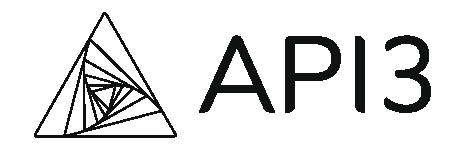
\includegraphics[width=0.7\textwidth]{fig/api3.pdf} \\ APIs Descentralizadas para la Web 3.0}
\author{Burak Benligiray, Sa\v{s}a Mili\'{c}, Heikki Vänttinen}
\date{\href{https://api3.org}{api3.org} \\ \medskip Septiembre 2020, v1.0.1}

% no paragraph indents
\setlength\parindent{0pt}
% vertical paragraph spacing
\setlength{\parskip}{1em}
% add dot after section number
\titlelabel{\thetitle.\quad}

\pagestyle{fancy}
\fancyhf{}
\lhead{\small API3: APIs Descentralizadas para la Web 3.0}
\rhead{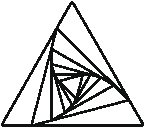
\includegraphics[height=7mm]{fig/api3-solo.pdf}}
\fancyfoot[C]{\thepage}

\begin{document}

\pagenumbering{gobble}

\maketitle

\begin{abstract}
\noindent 
Dado que las aplicaciones descentralizadas comienzan a prestar servicios significativos en esferas como las finanzas descentralizadas, existe una necesidad cada vez mayor de que estas aplicaciones reciban datos o desencadenen eventos utilizando las tradicionales API de la Web. Sin embargo, las soluciones genéricas de oráculo no abordan adecuadamente el problema de la conectividad de la API debido a un enfoque demasiado generalizado y equivocado. Para remediar este problema, la API3 impulsará un esfuerzo de colaboración para crear una nueva generación de API nativas de la cadena de bloques, descentralizadas, o dAPI para abreviar. Los dAPI están compuestos por oráculos de primera mano operados por proveedores de API y, por lo tanto, son más seguros y rentables que las soluciones alternativas que emplean intermediarios.  En el centro de la mecánica de gobernanza, seguridad y captura de valor de esta iniciativa estará el token de la API3.  El uso del token otorgará a sus titulares plenos derechos de gobierno sobre el DAO de la API3 junto con todas las recompensas asociadas.  Los tokens API3 depositados se utilizarán como garantía para el servicio de seguro de la cadena que proporcionará garantías de seguridad cuantificables y fiables a los usuarios de la DAPI.  Este empleo elimina la necesidad de una autoridad central a nivel del ecosistema.  Como resultado, el proyecto API3 permitirá que las plataformas de contratos inteligentes aprovechen las API para la construcción de aplicaciones significativas de una manera verdaderamente descentralizada y de confianza minimizada.
\end{abstract}

\newpage
\pagenumbering{roman}
\setcounter{page}{2}
\renewcommand{\contentsname}{} % no "contents" title
\tableofcontents


\newpage
\pagenumbering{arabic}
\setcounter{page}{1}

%~~~~~~~~~~~~~~~~~~~~~~~~~~~~~~~~~~~~~~~~~~~~~~~~~~~~~~~~~~~~~~~~~~~
\section{Introducción}
\label{sec:introduction}

Estamos presenciando el nacimiento de aplicaciones descentralizadas que son capaces de interactuar con el mundo real, lo que se refleja inmediatamente en el valor que adquieren. El ejemplo más destacado de este fenómeno es el reciente aumento del valor que fluye hacia el DeFi (financiación descentralizada) con más de 8.000 millones de dólares de valor total asegurado en varias aplicaciones a partir de septiembre de 2020 ~\cite{defipulse}.
Una aplicación de DeFi típicamente requiere que los precios de los activos sean transmitidos a su plataforma de contratos inteligentes a través de una alimentación de datos ~\cite{liu:2020}.
Esta alimentación de datos facilita la interacción de la aplicación con el mundo real, permitiéndole en última instancia proporcionar servicios significativos como intercambios de derivados y préstamos. Lo que se está desarrollando en este momento no es sólo el auge del DeFi, sino el auge de las aplicaciones descentralizadas que pueden interactuar de manera significativa con el mundo real, y el DeFi es sólo la punta del iceberg.


Las empresas ofrecen una amplia variedad de servicios a través de las APIs de la Web, que van desde proporcionar datos sobre el precio de los activos hasta la ejecución de transacciones financieras tradicionales. Es fundamental que las aplicaciones descentralizadas puedan acceder al tipo de servicios que ofrecen las API de la Web para interactuar con el mundo real, pero estas API no son compatibles de forma nativa con las aplicaciones descentralizadas. Las soluciones de interfaz existentes basadas en intermediarios son centralizadas, inseguras y costosas, y sólo se utilizan a falta de una alternativa mejor. Con la API3, nuestro objetivo es que el concepto de una API dé el siguiente paso evolutivo para cumplir los requisitos de descentralización inevitablemente estrictos de la Web 3.0 sin emplear intermediarios de terceros. Utilizaremos el término dAPI para referirnos a esta nueva generación de API descentralizadas.

Una dAPI es una solución segura y rentable para proporcionar un servicio API tradicional a los contratos inteligentes de forma descentralizada. Se compone de los siguientes elementos:
\begin{itemize}
    \item múltiples API, donde el término API no sólo se refiere a una interfaz técnica, sino a un servicio que proporciona una empresa del mundo real;
    \item una red descentralizada de oráculos de primera mano, es decir, oráculos operados por los propios proveedores de API;
    \item una entidad rectora descentralizada para supervisar la red de oráculos.
\end{itemize}

\begin{figure}[!t]
    \centering
    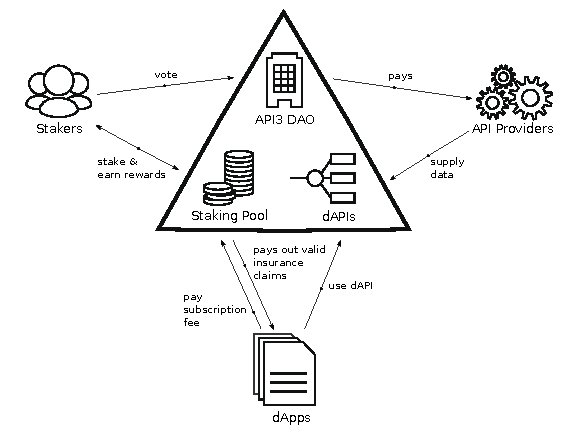
\includegraphics[width=0.9\textwidth]{fig/teaser.pdf}
	\caption{Visión general de la mecánica del API3.}
	\label{fig:teaser}
\end{figure}

La API3 es un esfuerzo de colaboración para crear, administrar y monetizar las dAPIs a escala. Para lograrlo de manera totalmente descentralizada, los incentivos de los participantes se conciliarán mediante las utilidades de gobernanza, seguridad y captura de valor del token de la API3. El proyecto tendrá un modelo de gobernanza completamente abierto y directo, en el que cualquier poseedor de un token API3 podrá participar para obtener privilegios de voto directo en el DAO API3. Además, los poseedores de tokens recibirán una porción de los ingresos de la dAPI, recompensas inflacionarias de staking y cualquier otro beneficio adicional que el DAO pueda decidir en el futuro. Las fichas API3 apostadas respaldarán un servicio de seguro en cadena como garantía para proporcionar a los usuarios de la dAPI garantías de seguridad cuantificables y sin necesidad de  confianza  (véase la Figura~\ref{fig:teaser}).

Uno de los defectos fundamentales de las soluciones de oráculo existentes es el intento de establecer y mantener una conexión parasitaria con las fuentes de datos, que no puede producir un ecosistema sostenible. Por el contrario, partimos del reconocimiento de que los proveedores de API son el motor de este Proyecto. Por lo tanto, no se les hará desaparecer, sino que se les atribuirá y compensará para que sus intereses estén totalmente alineados con los intereses del gran ecosistema API3. Ya hemos sido testigos del afán de los proveedores de API por incentivar la adopción de sus servicios por parte de las aplicaciones descentralizadas mediante el suministro de llamadas gratuitas a la red de pruebas para sus APIs de pago ~\cite{honeycomb.market}
y la oferta de premios en efectivo para los hackathons ~\cite{honeycomb-hackathon}.
El cultivo de esta cooperación será una de las principales fuentes de fortaleza de la API3.

Las soluciones descentralizadas de redes de oráculos emplean oráculos de terceros porque a menudo no es factible que los proveedores de API operen sus propios nodos de oráculos. Esto posiciona a los oráculos de terceros como intermediarios costosos y forma una superficie de ataque adicional.
 
Para eliminar estos problemas y hacer que los proveedores de API se comprometan aún más con el ecosistema, los datos de la API3 estarán compuestos por oráculos de primera línea operados por los proveedores de API. Esto será posible gracias a Airnode, un nodo oráculo sin servidores que está diseñado para no requerir conocimientos técnicos, mantenimiento o conservación por parte del proveedor de la API. Las dAPI resultantes serán rentables y seguras frente a los ataques de una capa intermedia de terceros.

En caso de mal funcionamiento, el usuario de la dAPI podrá reclamar una indemnización hasta una cantidad pre negociada de la reserva de stacks. Kleros~\cite{kleros:2019}, un protocolo de resolución de disputas en cadena, se utilizará para decidir si la reclamación debe ser pagada en base a las pruebas presentadas. Esto incentivará a los interesados a participar activamente en la gestión para garantizar que las dAPIs se gestionen de forma transparente y de manera que se reduzcan al mínimo los riesgos para la seguridad. Una gobernanza satisfactoria, que genere ingresos procedentes de las dAPIs y que al mismo tiempo evite los errores que se traduzcan en el pago de las reclamaciones de seguros, se recompensará con fichas API3, lo que creará un circuito de retroalimentación positiva que mejorará continuamente la gobernanza.

Consulte de nuevo la Figura~\ref{fig:teaser} para obtener una visión general de nuestra solución. Las dAPIs son redes de oráculos de primera instancia que proporcionan servicios tradicionales de API de forma descentralizada y nativa en la cadena de bloques. El DAO de la API3 construye, gestiona y monetiza las dAPIs a escala. Las aplicaciones descentralizadas pagan una cuota de suscripción para acceder a una dAPI. Las aplicaciones descentralizadas pagan una cuota de suscripción para acceder a una dAPI. Los poseedores de tokens API3 participan en un fondo común para recibir recompensas y derechos de voto en el DAO. Este fondo común se utiliza como garantía para un servicio de seguro en cadena que proporciona a los usuarios de dAPI un nivel de seguridad cuantificable. La API3 mejora las soluciones de oráculo existentes en cuanto a descentralización, eficiencia en función de los costos, seguridad, transparencia y potencial de crecimiento del ecosistema.

%~~~~~~~~~~~~~~~~~~~~~~~~~~~~~~~~~~~~~~~~~~~~~~~~~~~~~~~~~~~~~~~~~~~
\section{Problemas de conectividad de las APIs}
\label{sec:api-connectivity-problem}

Una interfaz de programación de aplicaciones (API) es un protocolo bien normalizado y documentado que se utiliza para comunicarse con una aplicación específica para recibir servicios de ella. Esos servicios pueden consistir en la recepción de datos o en la activación de un evento. Las aplicaciones pueden comunicarse entre sí a través de sus API, lo que permite integrarlas para construir aplicaciones más complejas. Por ello, las APIs se denominan el pegamento que mantiene unido el mundo digital.

Como resultado de que las empresas utilizan las APIs para monetizar sus datos y servicios, el concepto de una API ha trascendido su significado inicial. El término ya no se refiere a la implementación técnica de una interfaz, sino a un producto completo que incluye el servicio que envuelve~\cite{deloitte:2015}.
Las empresas mundiales que proporcionan API generan un promedio del $25\%$ de sus ingresos organizativos a partir de las APIs ~\cite{mulesoft:2019}.
Empresas como Sales-force, Expedia y eBay han declarado que generan la mayoría de sus ingresos a través de las APIs~\cite{iyer:2015},
y estamos en la cúspide de modelos de negocio totalmente centrados en las APIs ~\cite{ibm:2016}.
Se espera que incluso industrias arraigadas como la banca se vean perturbadas por este movimiento ~\cite{capgemini:2019a}.

La integración de los servicios existentes en sus aplicaciones a través de las APIs ha permitido a los desarrolladores crear aplicaciones cada vez más complejas y capaces, lo que ha dado lugar al surgimiento de gigantescos servicios web y aplicaciones móviles. Sin embargo, estas API a través de las cuales las empresas prestan sus servicios no son directamente compatibles con los contratos inteligentes debido a razones técnicas que se describirán en la Sección~\ref{sec:oracle-problem-a-misnomer}, lo que ha frenado el desarrollo de aplicaciones descentralizadas significativas. Por lo tanto, la dificultad a la que nos enfrentamos para construir aplicaciones descentralizadas que puedan interactuar con el mundo real puede describirse mejor en la actualidad como el problema de conectividad de las APIs. Una mala interpretación de este problema llevará a una solución no óptima.

\subsection{Problema del Oráculo: Una mala interpretación de la fuente-agnóstica.}
\label{sec:oracle-problem-a-misnomer}

La descentralización define la Web 3.0, que se caracteriza por distribuir la computación y establecer resultados a través de reglas de consenso predeterminadas ~\cite{nakamoto:2009}.
La lógica de negocio de una aplicación descentralizada se implementa como un contrato inteligente ~\cite{szabo:1994},
que se ejecuta en una plataforma de contratos inteligentes basado en la cadena de bloques ~\cite{buterin:2014a}.
La descentralización permite a los participantes cooperar sin necesidad de confianza mutua o de un tercero de confianza, y por lo tanto proporciona robustez contra los ataques y la censura.

Para hacer cumplir las reglas consensuadas, los nodos de la plataforma de contratos inteligentes tienen que verificar que cada solicitud de contrato ha dado lugar al resultado correcto repitiendo el cómputo localmente. Para que esto sea posible, los contratos inteligentes sólo pueden operar con información que sea accesible y acordada por todos los nodos de la plataforma del contrato inteligente. En términos más simples, los contratos inteligentes sólo pueden operar con la información que está fácilmente disponible en la cadena de bloques, y no pueden interactuar con el mundo exterior directamente. Esto es ampliamente conocido como el "problema del oráculo", refiriéndose a un agente idealizado que puede entregar un pedazo de verdad arbitrariamente definido la cadena de bloques.

El problema del oráculo está mal planteado, ya que incluso su nombre sugiere una solución imposible. Una analogía sería abordar el problema de ir del punto A al punto B como el "problema de la teletransportación". No obstante, la primera generación de soluciones intentó poner en práctica este oráculo literal planteando una pregunta y obteniendo su respuesta, lo que produce tiempos de resolución medibles en días y costos de gas extremos debido al número de transacciones que hay que hacer~\cite{augur:2019}, lo que no es ideal para casos de uso como el DeFi o los mercados de predicción. Debemos señalar que este enfoque es efectivamente adecuado si la información que se debe entregar es subjetiva. Un buen ejemplo sería la resolución de un litigio judicial ~\cite{kleros:2019}.

Las soluciones de segunda generación redujeron su alcance para cubrir sólo la información factual a la que se puede acceder mediante programación, y terminaron con el "problema de interoperabilidad". En estas soluciones, un nodo oráculo que se integra a dos sistemas arbitrarios (una cadena de bloques y una API, dos cadenas de bloques, etc.) actúa como un inter mediador automatizado entre los dos ~\cite{ellis:2017,band,depedro:2017,tellor}.
El uso de varios de estos nodos oráculo y el establecimiento del resultado mediante reglas de consenso predeterminadas proporciona garantías de seguridad que complementan la tecnología de la cadena de bloques subyacente.  Estas soluciones son más rápidas y menos costosas en comparación con los oráculos de origen colectivo y, por consiguiente, son viables para más casos de uso, aunque sufren de un diseño en torno a una generalización excesiva del problema en cuestión.

Las soluciones de interoperabilidad implican a tres partes: Los proveedores de API, los oráculos y los consumidores de datos ~\cite{benligiray:2019}.
Sin embargo, caen en el riesgo de modelar su ecosistema como compuesto únicamente por oráculos y consumidores de datos, mientras ignoran de dónde proceden los datos. En otras palabras, sus modelos tratan el nodo oráculo como el oráculo mítico que es la fuente de la verdad. El hecho de ser ciego a un tercio del problema de esta manera da lugar a soluciones poco prácticas que se perciben como factibles.

El hecho de que la solución de interoperabilidad sea agnóstica a la fuente da como resultado las siguientes consecuencias:
\begin{itemize}
    \item Una capa intermedia de oráculos de terceros inseguros y costosos, que podría haber sido reemplazada por oráculos operados por proveedores de API;
    \item Un ecosistema que alimenta a los intermediarios que buscan rentas, mientras que excluye las fuentes activas de los datos;
    \item Tratamiento indiscriminado de los datos recibidos de diferentes fuentes en una alimentación de datos.
\end{itemize}

Otro problema generalizado de las soluciones de interoperabilidad es que, al tratarse de protocolos de bajo nivel, consideran la interfaz como un componente técnico, o \textit{middleware}, en lugar de un producto completo. Como efecto secundario, el gobierno de la interfaz queda fuera de alcance.   Sin embargo, la gobernanza no es un problema trivial, porque una interfaz descentralizada requiere la cooperación de partes independientes y competidoras. La solución que se utiliza actualmente es una entidad centralizada de confianza para gobernar la interfaz, lo que está en desacuerdo con el objetivo principal de la descentralización.  La entidad gobernante tiene pleno control sobre la producción de una red de oráculos, lo que significa que una red de oráculos descentralizada con gobierno centralizado es un oráculo centralizado con pasos adicionales.

\subsection{APIs Descentralizadas}
\label{sec:decentralized-apis}

Los problemas de la generación anterior de soluciones de interoperabilidad sólo pueden resolverse adoptando una nueva perspectiva: El problema que se plantea es, en esencia, el de que las aplicaciones descentralizadas no pueden recibir servicios de los proveedores de API tradicionales de manera descentralizada. De hecho, el uso principal de las soluciones de interoperabilidad hoy en día es proporcionar precios de activos corregidos desde las APIs de intercambio centralizadas hasta las aplicaciones DeFi, y los casos de uso emergentes como los mercados de predicción ~\cite{omen} 
y el seguro paramétrico ~\cite{capgemini:2019b} tienen todos requisitos similares. 
Por lo tanto, si se especifica más la definición del problema como tal, nos permitirá llegar a la próxima generación de soluciones de interconectividad en el mundo real. 

\begin{figure}
     \centering
     \begin{subfigure}{0.49\textwidth}
        \centering
         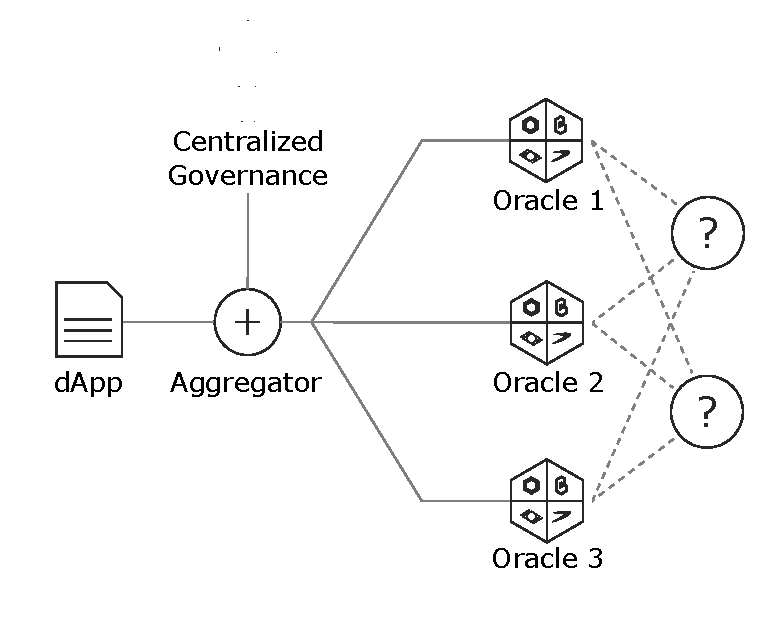
\includegraphics[height=5.7cm]{fig/solutions-comparison-a.pdf}
         \caption{Solución de interoperabilidad descentralizada}
         \label{fig:solutions-comparison-3rd}
     \end{subfigure}
     \hfill
     \begin{subfigure}{0.49\textwidth}
        \centering
         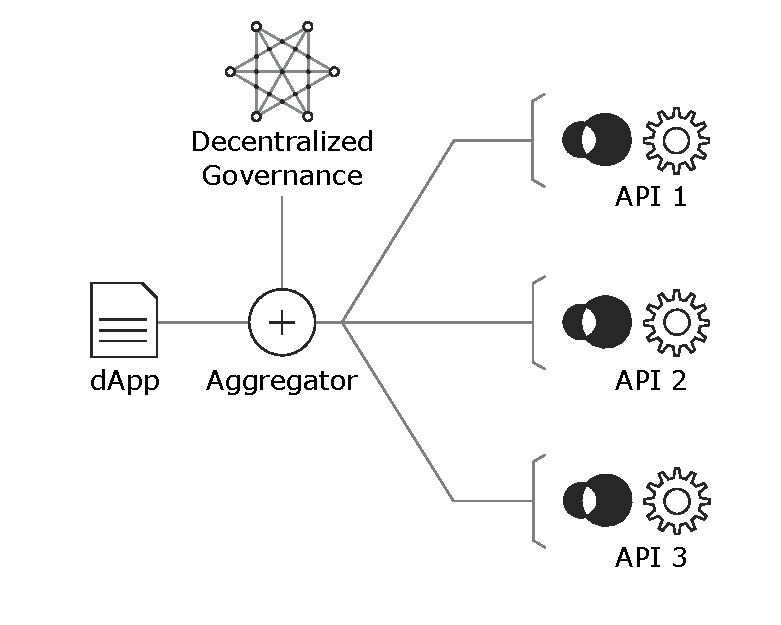
\includegraphics[height=5.7cm]{fig/solutions-comparison-b.pdf}
         \caption{API descentralizada (dAPI)}
         \label{fig:solutions-comparison-1st}
     \end{subfigure}
     \caption{DLas soluciones de interoperabilidad descentralizadas emplean oráculos de terceros que no revelan sus fuentes de forma nativa. Las dAPIs se componen de oráculos de primera mano, lo que significa que los proveedores de API operan sus propios nodos aéreos. Además, las dAPIs están descentralizados en cuanto a la forma en que se rigen, lo que da lugar a una descentralización de extremo a extremo. }
    \label{fig:solutions-comparison}
\end{figure}

TEsta nueva definición del problema implica que las aplicaciones descentralizadas requieren que se presten servicios específicos de API de la Web a la cadena de bloques y que esto se haga de manera totalmente descentralizada, rentable y segura. La determinación de los requisitos nos permite diseñar un producto completo que los satisfaga de manera óptima: Las APIs descentralizadas, o dAPI para abreviar, son redes de oráculos de primera parte operados por proveedores de API que se rigen de forma descentralizada. Por el contrario, las soluciones de interoperabilidad descentralizadas consisten en una red de oráculos de terceros intermediarios gobernados por una entidad centralizada, lo cual es necesario por su definición de problemas poco especificada.
Véase la Figura~\ref{fig:solutions-comparison} fpara una comparación visual. 

%~~~~~~~~~~~~~~~~~~~~~~~~~~~~~~~~~~~~~~~~~~~~~~~~~~~~~~~~~~~~~~~~~~~
\section{Problemas con los Oráculos de Terceros como Intermediarios}
\label{sec:issues-with-third-party-oracles-as-middlemen}

Las soluciones existentes prevén un problema abstracto en el que un sistema arbitrario necesita poder interoperar con otro sistema arbitrario a través de sus interfaces técnicas en un sentido muy general. Esta generalidad excesiva requiere una interfaz siempre flexible que sólo puede ser soportada por oráculos de terceros. Sin embargo, esta solución no es óptima porque el alcance práctico del problema es mucho más limitado. En la mayoría de los casos, el problema de la interoperabilidad descentralizada es en realidad el problema de recibir servicios de los proveedores de API tradicionales de manera descentralizada. Esta definición más limitada del problema permite soluciones óptimas que no requieren una capa intermedia de terceros en el trayecto de la interfaz. A lo largo del resto de esta sección, analizaremos las consecuencias de confiar en los intermediarios como parte de una solución de interoperabilidad.

\subsection{Vulnerabilidades}
\label{sec:vulnerability}

Una red descentralizada de oráculos utiliza una función de agregación para reducir los informes de los oráculos a una sola respuesta. Esta función es esencialmente un algoritmo de consenso y, como todos los algoritmos de consenso, es susceptible a una cierta proporción de actores deshonestos. Esto significa que un grupo de oráculos maliciosos pueden confabularse para sesgar el resultado, e incluso controlarlo completamente. Además, un solo actor puede fabricar múltiples identidades de operadores de nodos oráculos -así como construir un historial suficiente de operaciones honestas- para realizar los mismos tipos de ataques completamente por sí mismos, lo que se conoce como un ataque Sybil ~\cite{douceur:2002}.

La desventaja más importante de tener una capa adicional de partes en el camino de la interfaz es la formación de superficies de ataque completamente nuevas. Esto significa que cada capa adicional de intermediarios podría ejecutar la colusión y los ataques de Sybil descritas anteriormente de forma independiente. Entonces, en términos de seguridad, la solución definitiva es la eliminación completa de los intermediarios.

\subsection{Impuestos de Intermediarios}
\label{sec:middleman-tax}

\begin{figure}
    \centering
	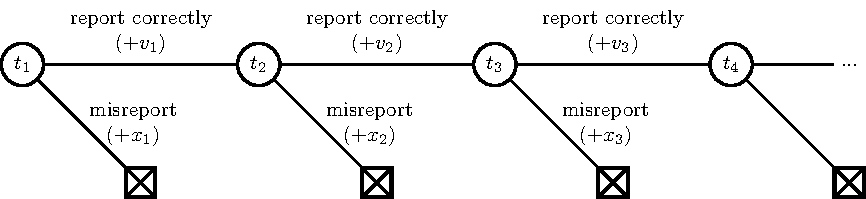
\includegraphics[width=\textwidth]{fig/decision-tree.pdf}
	\caption{Un árbol de decisiones que describe las acciones que un oráculo puede tomar y sus resultados. En una transacción determinada $t_i$, un oráculo puede informar honestamente y ganar $v_i$ o informar mal y ganar $x_i$. Una acción deshonesta hace que el oráculo deje de ser utilizado, es decir, que se ponga fin al juego. .}
	\label{fig:decision-tree}
\end{figure}

Un oráculo juega un juego en el que pueden informar con honestidad o informar mal (lo que incluye negar el servicio). Informar honestamente sólo tiene un beneficio adicional, pero permite al oráculo seguir jugando el juego. Por otro lado, la presentación de informes erróneos tiene un pago único proporcional al valor asegurado por los contratos, dependiendo del informe, pero da lugar a que el juego termine  (véase la Figura~\ref{fig:decision-tree}).
Entonces, la máxima retribución acumulada que el oráculo puede recibir a partir de la transacción $t_i$es. 

\begin{equation}
P \left[ i \right] = \max \left( x_i, v_i + P \left[ i + 1 \right] \right).
\end{equation}

Un oráculo racional eventualmente informará erróneamente si la cantidad que puede obtener de un ataque supera las ganancias potenciales que puede hacer si no realiza el ataque. Es decir, si lo siguiente es válido para un oráculo racional dado, eventualmente informará erróneamente:

\begin{equation}
\exists i \in \mathbb{N},~ x_i > v_i + P \left[ i + 1 \right].
\end{equation}

Esto indica que el beneficio potencial que un oráculo obtendrá al actuar con honestidad debe superar la cantidad que puede obtenerse de una información errónea en todo momento para evitar cualquier tipo de información errónea. Aunque se puede aproximar $v$ con la cantidad pagada al oráculo por solicitud y $x$ con la cantidad que se asegura con la respuesta del oráculo, esto subestimaría el riesgo porque hay factores adicionales que inclinan a los oráculos hacia la notificación errónea, algunos de los cuales se indican a continuación:

\begin{itemize}
    \item Según la teoría de la preferencia temporal y~\cite{frederick:2002}, el operador del nodo del oráculo valorará menos las recompensas futuras (es decir, $v_i$ decae al aumentar $i$).
    \item En la práctica, el oráculo actuando honestamente no garantiza que el juego continúe y este riesgo disminuye aún más el valor de las recompensas futuras.
    \item Puede haber beneficios adicionales al realizar un ataque que no se contabilizan, por ejemplo, la apertura de una posición corta en un activo que se depreciará con el fracaso de la solución del oráculo.
\end{itemize}

Debido a esta incertidumbre, es necesario sobreestimar el $v_i$ necesario, es decir, pagar en exceso al oráculo para que no ataque.

Este modelo puede extenderse a las redes descentralizadas de oráculos. Dado que los informes de los oráculos o sus artefactos se registran en cadena, es trivial implementar un contrato inteligente que recompense a los oráculos confabulados sin necesidad de confianza. Esto significa que un tercero que pueda beneficiarse de un ataque puede emplear oráculos con la garantía de que se les pagará una cantidad determinada si se confabulan.

En un alto nivel, el trabajo de un oráculo es esencialmente: (1) escuchar las peticiones on-chain, (2) hacer las respectivas llamadas API off-chain, y (3) escribir la respuesta de nuevo en la cadena. Por lo tanto, un oráculo de terceros es fundamentalmente un intermediario. Aunque el servicio prestado es el mínimo posible, estos intermediarios tienen que ser pagados proporcionalmente a la cantidad que está siendo asegurada por la alimentación de datos debido a las razones descritas anteriormente, lo cual es especialmente problemático para casos de uso de alto valor como el DeFi. Llamamos a este fenómeno el "impuesto de intermediarios", que puede eliminarse completamente evitando los oráculos de terceros, lo que supone un ahorro de costes muy importante para los usuarios.

\subsection{Redundancia Ineficaz}
\label{sec:ineffective-redundancy}

\begin{figure}
    \centering
    \begin{subfigure}{0.513398876\textwidth}
         \centering
         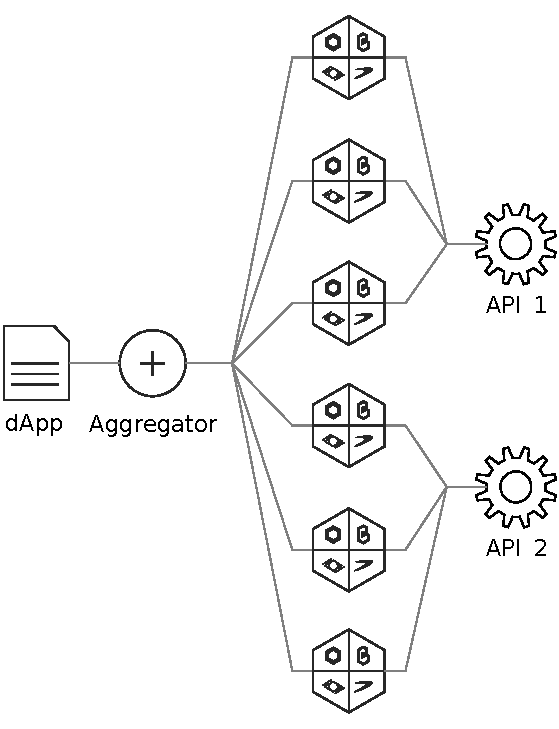
\includegraphics[height=8cm]{fig/oracle-level-decentralization-a.pdf}
         \caption{Alimentación de datos compuesta por oráculos de terceros }
         \label{fig:oracle-level-decentralization-a}
     \end{subfigure}
     \hfill
     \begin{subfigure}{0.466601124\textwidth}
         \centering
         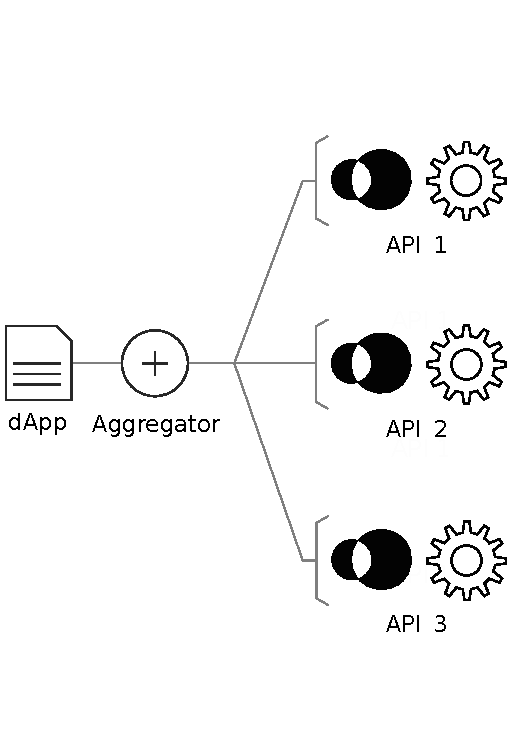
\includegraphics[height=8cm]{fig/oracle-level-decentralization-b.pdf}
         \caption{Alimentación de datos compuesta por oráculos de primera mano }
         \label{fig:oracle-level-decentralization-b}
     \end{subfigure}
	\caption{El uso de oráculos de terceros requiere una descentralización excesiva a nivel de oráculo, mientras que los oráculos de primera mano proporcionan un mejor grado de descentralización de manera más segura y eficaz en función de los costos.}
	\label{fig:oracle-level-decentralization}
\end{figure}

La alimentación de los datos en función de oráculos de terceros requiere una redundancia excesiva a nivel de oráculo (véase la Figura~\ref{fig:oracle-level-decentralization}).
Ello se debe a que los oráculos de terceros son mucho menos fiables que los proveedores de API, ya que estos últimos tienen un negocio tradicional off-chain y una reputación que mantener. Por lo general, cada proveedor de API cuenta con dos o tres oráculos en ese tipo de alimentación de datos. Obsérvese que esta descentralización no proporciona seguridad adicional a nivel de la fuente de datos, sino que sólo disminuye la vulnerabilidad adicional causada por la utilización de oráculos de terceros. Lamentablemente, esto da lugar a que los costos de operación se multipliquen en muchos niveles. Por ejemplo, la alimentación de datos emplea esencialmente a todo el personal técnico que opera los nodos del oráculo, y tener más de estos nodos significa apoyar a más personas. Además, el uso de más oráculos da lugar a un aumento directo de los costos del gas. Concretamente, los costos del gas de solicitud-respuesta del oráculo aumentan linealmente con el número de oráculos, mientras que los costos del gas de las funciones de agregación que realizan operaciones combinadas (por ejemplo, la mediana) aumentan superlinealmente.

\subsection{Falta de Transparencia}
\label{sec:lack-of-transparency}

La descentralización a nivel de la API y la descentralización a nivel de oráculo son interdependientes entre sí; el sistema general está tan descentralizado como el más centralizado de los dos, es decir, el eslabón más débil. Sin embargo, el público en general e incluso los usuarios de las redes descentralizadas de oráculos pasan por alto este hecho y confunden la descentralización a nivel de oráculo con la descentralización general del sistema. Esto se debe principalmente a la falta de transparencia en lo que respecta a las fuentes de datos utilizadas por los oráculos ~\cite{feeds.chain.link}, lo que oculta el hecho de que la descentralización se ve gravemente obstaculizada a nivel de las fuentes de datos (API).

Las fuentes de datos compuestas por oráculos de terceros parecen más descentralizadas de lo que realmente están.  Además, cuando los alimentadores de datos no son transparentes en cuanto a la fuente de sus datos, los desarrolladores no pueden evaluar la integridad de los alimentadores de datos y tienen que confiar en la entidad gobernante. Sin embargo, no existe un incentivo inmediato para que la entidad rectora elija la calidad en lugar de los precios más bajos y la conveniencia si las fuentes de datos no son transparentes, lo que puede dar lugar al resultado comúnmente denominado "basura que entra, basura que sale".

Curiosamente, lo que es una táctica favorable para la entidad gobernante, es decir, oscurecer la fuente de datos, es muy necesario para los oráculos de terceros. La mayoría de las condiciones de servicio de la API prohíben la reventa o la distribución no autorizada de los datos de la API, lo que hace que el operador de un nodo oráculo que presta servicios a esas API incumpla esas condiciones y sea susceptible de amplias fuentes de responsabilidad legal, incluidas las reclamaciones del proveedor de la API~\cite{data-licensing}.
Esta cuestión se ve agravada por los tiempos de respuesta y de llamada a la API, así como por los pagos que se registran en una cadena de bloqueo pública. Esto no sólo pone a los operadores de nodos individuales en riesgo de litigio, sino que también crea un riesgo sistémico para toda la red de oráculos, ya que una acción legal coordinada a escala pondría a los oráculos de terceros existentes fuera de servicio inmediatamente y desalentaría la incorporación de otros nuevos. 

Obsérvese que, aunque la falta de transparencia y la abstracción de las fuentes de datos es la norma, no es en absoluto una necesidad. Especialmente cuando el proveedor de la API y los incentivos del ecosistema están alineados, es perfectamente posible que los oráculos sirvan los datos de la API a los usuarios con el consentimiento expreso del proveedor de la API, permitiendo que los oráculos revelen sus fuentes de datos a sus usuarios~\cite{honeycomb.market}.
A los proveedores de API les interesa hacer esto, ya que aumenta la demanda de sus datos on-chain.

%~~~~~~~~~~~~~~~~~~~~~~~~~~~~~~~~~~~~~~~~~~~~~~~~~~~~~~~~~~~~~~~~~~~
\section{Airnode: Un nodo diseñado para los Oráculos de Primera Mano}
\label{sec:airnode-a-node-designed-for-first-party-oracles}

Los oráculos de primera mano son parte integral de la solución API3. Esto significa que cada API está servida por un oráculo que es operado por la entidad que posee la API, en lugar de un tercero. En esta sección, analizaremos las ventajas de utilizar oráculos de primera mano, por qué no es factible que los proveedores de API operen sus propios oráculos con las soluciones disponibles en la actualidad, y cómo pretendemos resolver este problema con Airnode.

\subsection{Beneficios de la desintermediación}
\label{sec:benefits-of-disintermediation}

Existe una solución sencilla para todos los problemas tratados en la Sección~\ref{sec:issues-with-third-party-oracles-as-middlemen}: oráculos de primera mano, es decir, oráculos operados por los propios proveedores de API. Los proveedores de API que operan sus propios oráculos significan que firmarían sus respuestas con sus claves privadas a nivel del protocolo de la plataforma de contratos inteligentes, lo que constituye la mejor prueba de que los datos no han sido manipulados. Además, los oráculos de primera mano son privados por defecto, ya que un tercero no puede observar los datos en bruto de la API que se están procesando, lo que permite utilizarlos en una mayor variedad de casos de uso de forma nativa. 

Una alimentación de datos compuesta por oráculos de primera mano sería más rentable en comparación con una que emplee intermediarios, ya que es necesario pagar a los intermediarios tanto por sus servicios como para incentivarlos a no atacar la alimentación de datos (lo que se denomina el impuesto de intermediarios en la Sección ~\ref{sec:middleman-tax}).
Además, una alimentación de datos compuesta de oráculos de primera mano necesitará menos oráculos, ya que no necesitaría una descentralización excesivamente redundante a nivel de oráculo para protegerse contra los ataques de terceros. Suponiendo que cada API suele contar con el servicio de al menos dos oráculos de terceros, la alimentación de datos alimentada por oráculos de primera parte sería al menos un $50\%$ más eficiente en términos de costos de gas, según una estimación conservadora.


Los oráculos de primera mano también proporcionan la tan necesaria transparencia en cuanto a los datos fuente y el grado de descentralización. Dado que cada proveedor de API operará un oráculo -que será visible on-chain-, el número de oráculos que sirvan para alimentar los datos representará con precisión el grado de descentralización, ya que existe un mapeo individual entre el oráculo y la fuente de datos. Además, los proveedores de API publicarían sus identidades on-chain a través de canales off-chain, lo que permitiría a los usuarios verificar qué datos están consumiendo en un momento dado.

Por último, el hecho de que los proveedores de API operen los oráculos resuelve los problemas jurídicos mencionados en la Sección~\ref{sec:lack-of-transparency}, aya que los servicios de API ya no necesitan ser licenciados a un tercero y los proveedores de API reciben la totalidad de los ingresos. Además, esto resuelve el problema de la búsqueda de rentas de oráculos de terceros, y permite que los fondos se redirijan al grupo que está haciendo el trabajo pesado, los proveedores de API. Al incentivar a los proveedores de API se alinean sus intereses financieros con los del ecosistema de API3, lo que da lugar a un fuerte vínculo mutuo entre ambos.

\subsubsection{Firma de datos Off-chain}
\label{sec:off-chain-signing-of-data}

Hay una solución híbrida que todavía depende de oráculos de terceros, pero que no les permite manipular los datos. En este esquema, el proveedor de la API firma sus datos con su clave privada off-chain y la suministra a través de un punto final de la API normal. Los oráculos de terceros llaman a este punto final para obtener los datos firmados y publicarlos en la cadena. La autenticidad de los datos -que no son manipulados por los oráculos de terceros- puede verificarse entonces en la cadena utilizando la clave pública del proveedor de la API~\cite{open-price-feed}.

Aunque elimina el riesgo de alteración de los datos a nivel de oráculo, esta solución es esencialmente una medida a medias. Al depender de oráculos de terceros, sigue sufriendo los problemas de ecosistema causados por la dependencia de oráculos de terceros y, además, requiere modificaciones en el lado de la API para implementar la firma off-chain. Esto da lugar a una selección de API muy limitada, incluso en comparación con las soluciones habituales basadas en oráculos de terceros, y restringe el potencial de crecimiento del ecosistema de la solución a la escala de la aplicación

\subsection{Barreras para los proveedores de las APIs que operan oráculos}
\label{sec:barriers-to-api-providers-operating-oracles}

Durante nuestro trabajo en el Mercado de API de Honeycomb ~\cite{benligiray:2019} 
en los últimos dos años, nos comunicamos con los proveedores de API ampliamente y observamos las siguientes barreras para el abordaje y funcionamiento del oráculo:

\begin{enumerate}
    \item Los proveedores tradicionales de API no suelen estar más familiarizados con las tecnologías de la cadena de bloques que el público en general. Esto se aplica incluso a los que se encargan de la conservación de datos del mercado de la criptodivisa, ya que su principal operación consiste en recopilar datos de las APIs de intercambio, procesarlos y servir el resultado a través de sus propias API, lo que no requiere ningún conocimiento específico de la cadena de bloques. Por lo tanto, normalmente no pueden hacer funcionar fácilmente un nodo oráculo con recursos propios.
    \item No hay un mercado de trabajo para los operadores de los nodos oráculos. Incluso si algunos proveedores de API obtuvieran los conocimientos técnicos específicos necesarios contratando a los pocos operadores de nodos disponibles, no sería una solución escalable.
    \item El funcionamiento de un nodo oráculo consume muchos recursos en forma de horas-hombre y costes de infraestructura. A menos que se le garanticen subsidios significativos o ganancias futuras, operar un nodo oráculo es financieramente inviable.
    \item Operar un nodo oráculo requiere que el proveedor de la API realice transacciones con cryptodivisas. Específicamente, deben pagar los costos de gas en la moneda nativa (por ejemplo, ETH) y recibir pagos en una o más criptodivisas. Esto descalifica a la gran mayoría de los proveedores de API por razones de cumplimiento, legales y contables. Además, cualquier esquema que requiera que los proveedores de API participen en los fondos se rechaza categóricamente por razones similares relacionadas con el riesgo financiero.
\end{enumerate}

\subsection{Características del Airnode}
\label{sec:airnode-features}

\begin{figure}
    \centering
	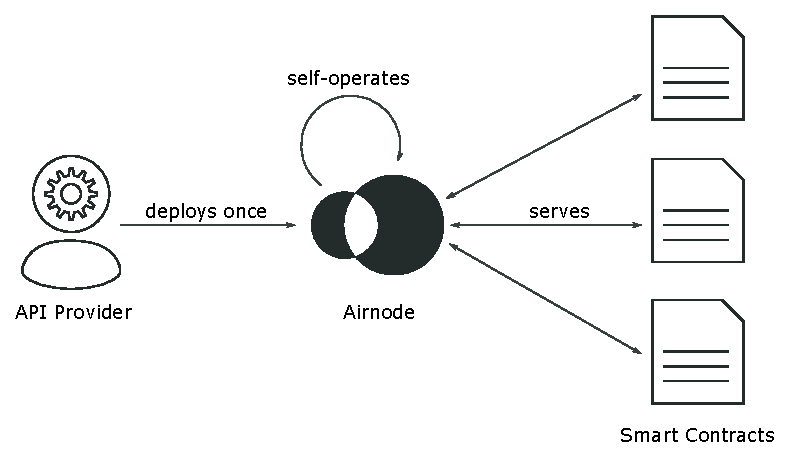
\includegraphics[width=0.8\textwidth]{fig/airnode.pdf}
	\caption{El Airnode está diseñado para ser desplegado una vez por el proveedor de la API, luego no requiere ningún otro mantenimiento.}
	\label{fig:airnode}
\end{figure}

Airnode es un nodo oráculo completamente sin servidores que está diseñado específicamente para que los proveedores de API operen sus propios oráculos (véase la Figura ~\ref{fig:airnode}).
Aborda todos los problemas relacionados con el nodo oráculo en la Sección ~\ref{sec:barriers-to-api-providers-operating-oracles}:

\begin{enumerate}
    \item No requiere ningún conocimiento específico para operar.  De hecho, es difícil incluso hablar de una operación, ya que el Airnode está diseñado para ser completamente \textit{ajustado y olvidar}.
    \item No requiere ningún mantenimiento diario, como la actualización del sistema operativo o la supervisión del nodo para el tiempo de funcionamiento, debido a la tecnología sin servidor totalmente gestionada existente. Está diseñado para ser apátrida, lo que lo hace extremadamente resistente a cualquier problema que pueda causar un tiempo de inactividad permanente y requerir la intervención del operador del nodo.
    \item Se basa en servicios de precio a la carta, lo que significa que al operador del nodo se le cobra sólo lo que se utiliza su nodo. Esto permite a cualquier proveedor de API ejecutar un oráculo de forma gratuita y empezar a pagar sólo después de que empiecen a generar ingresos.
    \item No requiere que el operador de nodo maneje en absoluto la criptodivisas. Su protocolo está diseñado de manera que el solicitante cubra todos los costes de gas.
\end{enumerate}

Una forma de ver Airnode es como un envoltorio ligero alrededor de una API Web que le permite comunicarse con plataformas de contratos inteligentes sin fricción de gastos generales o de pago de tokens. En cuanto al nivel de participación requerido del proveedor de la API, el uso de Airnode puede compararse con la utilización de una puerta de enlace de la API que hace que ésta sea accesible a través de la Web, en lugar de operar un nodo de la cadena de bloques como un negocio secundario. De hecho, nuestro objetivo es que Airnode se convierta en algo tan ubicuo y mundano para las APIs como el uso de una puerta de enlace de API, lo que hará que una gran variedad de oráculos de primera mano estén disponibles para la API3.

Los proveedores de API invierten importantes recursos para construir una infraestructura de alta disponibilidad. Por lo tanto, es importante que la implementación del nodo oráculo no contenga puntos únicos de fallo que puedan causar un tiempo de inactividad. Las soluciones existentes que utilizan oráculos de terceros dependen de la sobre redundancia a nivel de oráculo para cubrir esto, lo que resulta en costos excesivos como se menciona en la Sección~\ref{sec:ineffective-redundancy}.
La API3 prevé que cada API sólo sea atendida por su oráculo de primera mano, lo que significa que la redundancia tiene que ser implementada a nivel del Airnode individual. El hecho de que el nodo no tenga servidores permite que esto se haga fácilmente en diferentes zonas de disponibilidad de un solo proveedor de nubes, o incluso en múltiples proveedores de nubes. Cabe mencionar también que será posible contener el Airnode y operarlo en las instalaciones, aunque se recomendará el uso de la versión sin servidores en casi todos los casos de uso.

Airnode es desarrollado por los miembros fundadores de API3 y ahora es de código abierto\footnote{\url{https://github.com/api3dao/airnode}}. El software tiene todas las características del protocolo descrito en la Sección~\ref{sec:airnode-protocol} y su desarrollo será financiado por la API3 en forma de subsidios.

\subsection{Protocolo de los Airnode}
\label{sec:airnode-protocol}

De manera similar a como preferimos el problema de conectividad de la API mejor especificado sobre el problema del oráculo, creemos que un nodo oráculo debería estar diseñado para interconectar muy bien las APIs con las plataformas de contratos inteligentes, en lugar de ser una caja de arena que pueda pretender ser utilizada para cualquier propósito imaginable. Basándose en esta filosofía, el protocolo Airnode está diseñado para seguir los patrones de auto emergencia utilizados por las APIs para lograr una interfaz de plataforma de contratos inteligentes API tan transparente y sin fricciones como sea posible.

El primer estilo de API, y el más comúnmente utilizado, sigue el patrón de solicitud-respuesta, en el que el usuario hace una solicitud con parámetros y la API responde lo antes posible. Este será el primer patrón que Airnode soportará, ya que es fácil de estandarizar e integrar con las APIs existentes que siguen el mismo patrón. Un ejemplo de caso de uso de este esquema sería solicitar el resultado de una coincidencia específica que se entregará, lo que puede utilizarse para realizar predicciones de un mercado respectivo. Además, se prevé que Airnode apoye el patrón de publicación-suscripción, en el que el usuario solicita al oráculo que vuelva a llamar a un método específico cuando se cumplan las condiciones parametrizadas. Por ejemplo, una bolsa descentralizada puede solicitar al oráculo que desencadene un evento de liquidación para un usuario en una posición de apalancamiento cuando el precio de la ETH caiga por debajo de los 400 dólares. Cualquiera de estos patrones puede utilizarse para implementar las fuentes de datos en vivo que las aplicaciones de DeFi utilizan hoy en día ~\cite{liu:2020}, pero también pueden soportar una variedad mucho mayor de casos de uso en forma de dAPI.

Como se mencionó en la Sección~\ref{sec:airnode-features}, el protocolo Airnode está diseñado de tal manera que el solicitante asume todos los costos del gas, incluso las transacciones de cumplimiento de la solicitud. Esto se logra mediante que cada Airnode tenga una billetera separada para cada solicitante, de manera similar a como los intercambios de criptodivisas designan automáticamente las billeteras para que los usuarios depositen fondos en ellas. El solicitante financia esta cartera con la moneda nativa (por ejemplo, ETH), ya sea en una suma global o mediante microtransacciones por solicitud. Los fondos de esta billetera se utilizan para cumplir con todas las siguientes solicitudes hechas por el solicitante. Este plan tiene ventajas significativas:

\begin{itemize}
    \item La volatilidad de los costos del gas y de los precios de las fichas de pago (por ejemplo, LINK) hace que sea prácticamente imposible para los oráculos fijar precios rentables pero competitivos. Cal cular los precios dinámicamente en cadena requiere múltiples alimentaciones de datos y añade una importante sobrecarga de gas por solicitud. Con el protocolo Airnode, los proveedores de API no tienen que preocuparse por los costos del gas y pueden utilizar esquemas de precios como el de 0,1 dólares por llamada o el de 100 dólares al mes, que es similar a los modelos típicos de fijación de precios de la API.
    \item Como se mencionó en la Sección \ref{sec:barriers-to-api-providers-operating-oracles}, no es razonable esperar que los proveedores de API sean capaces de convertir el fiat en criptomoneda y financiar sus carteras de nodos como un parte de sus operaciones diarias. En este esquema, el operador del nodo nunca tiene que pensar en el balance de su cartera de nodos.
    \item Como se ha visto en un reciente ataque realizado a los suministros de datos Chainlink ~\cite{chainlink-gastoken}, los nodos oráculos que utilizan una wallet común para satisfacer las solicitudes son susceptibles de que los atacantes envíen solicitudes para vaciar sus carteras. La solución a esto es que los operadores de los nodos mantengan una lista blanca de direcciones de confianza de las que aceptarán peticiones. Además de la dificultad de determinar qué contratos se supone que son de confianza en este contexto, esto hace que cualquier tipo de servicio de listas públicas sea prácticamente inviable. Esta es una cuestión crítica, ya que detiene el escaso crecimiento independiente del ecosistema que está muerto en su camino. El nodo aéreo no es susceptible a este tipo de ataque, ya que la cartera designada de un solicitante sólo se utiliza para satisfacer las solicitudes de dicho solicitante, y no puede ser drenada por otros.
    \item Los nodos oráculos tradicionales tienen que satisfacer todas las solicitudes con precios de gas muy altos, ya que no pueden tolerar que su cola de transacciones sea bloqueada por una sola transacción hecha con un precio de gas bajo. Con el protocolo Airnode, esto ya no es una preocupación, ya que cada solicitante tendrá una cola de transacciones separada. Entonces, los solicitantes cuyas peticiones no sean críticas en cuanto al tiempo podrán proporcionar el precio del gas de cumplimiento como parámetro de la petición y disfrutar del servicio a un coste de gas mucho más bajo. Se puede esperar que este esquema tenga sinergia con el EIP1559~\cite{eip1559}.
\end{itemize}

Por último, mencionemos brevemente cómo el protocolo Airnode se aproxima a la monetización.    Es común que se trabaje con un token específico para un proyecto en el núcleo del protocolo en un intento de asegurar que dicho token sea necesario.   Sin embargo, esto induce una enorme sobrecarga del precio del gas, restringe severamente las opciones alternativas de monetización y crea una fricción general. Por estas razones, el protocolo Airnode evita a propósito el uso de dicho token. En su lugar, se permite al operador del nodo asociar contratos de autorización personalizados a sus puntos finales de oráculo, que en esencia deciden si se debe responder a un solicitante en base a cualquier criterio que se pueda aplicar on-chain. Los contratos de autorización pueden utilizarse para hacer cumplir las listas blancas, las listas negras, los pagos de suscripción mensual o las tasas por solicitud. Este esquema es muy flexible y se aplica de manera que no añade ningún gasto de gas.  Aunque la monetización de la dAPI es un asunto completamente independiente, la flexibilidad que proporciona Airnode se trasladará, por ejemplo, será posible implementar una dAPI en la que los usuarios asuman todos los costos del gas, lo que no es posible con las soluciones de oráculo existentes

\subsection{API integrations}
\label{sec:api-integrations}

Hay un problema del huevo y la gallina cuando se trata de integrar las APIs a los oráculos. Si no hay demanda existente de una API en un ecosistema de oráculo, nadie se ve incentivado a hacer la integración. Si la API no está disponible debido a la falta de integración, nadie desarrolla aplicaciones que creen la demanda. Esto se identificó como un punto de fricción clave para el ecosistema de los chainlink, y se propuso como solución Honeycomb API Marketplace~\cite{benligiray:2019}, que lleva más de un año en funcionamiento~\cite{honeycomb.market}.
Honeycomb ha integrado un gran número de API de primera clase a los oráculos Chainlink y, como resultado, este mercado sirve a una variedad de API que no tiene parangón en ningún ecosistema de oráculos.

Honeycomb utiliza un adaptador externo universal y un método novedoso para integrar las APIs a los oráculos Chainlink de forma declarativa, sin necesidad de escribir ningún código. Este método es superior al desarrollo de un adaptador externo para cada operación de la API~\cite{external-adapters} ya que sus integraciones son más rápidas, menos propensas a errores y pueden ser realizadas por personas no expertas. Utilizando estas herramientas patentadas, Honeycomb fue capaz de integrar cientos de operaciones de API únicas en unos pocos meses, lo que empequeñece a la competencia más cercana en un orden de magnitud.

Para que el API3 alcance su máximo potencial, necesitará cientos, si no miles de oráculos de primera mano para poder configurar fácilmente nuevos dAPI o recomponer los existentes. Esto sólo puede lograrse si las APIs pueden integrarse a Airnode de una manera aún más escalable. Con este fin, una versión mejorada de las herramientas de integración propietarias descritas anteriormente será de código abierto para Airnode. Tomando prestado del formato de la especificación OpenAPI ~\cite{oas}, las especificaciones de integración del oráculo (OIS) definen las operaciones de una API, los puntos finales de un oráculo, y cómo ambos se mapean entre sí.  Un usuario de Airnode podrá suministrar una API sobre su oráculo simplemente proporcionando su OIS a su nodo. Las integraciones realizadas en este formato estandarizado serán muy fáciles de recopilar, versionar y distribuir.

OIS es un archivo JSON, diseñado principalmente para describir las especificaciones de integración para el uso de Airnode. Esto significa que no pretende ser legible para los humanos primero y crearlo manualmente para especificar una integración sería difícil. Este problema se resolverá mediante ChainAPI, una plataforma de integración que permitirá a los usuarios generar OIS para sus API a través de una interfaz gráfica fácil de usar. Esto irá acompañado de otras mejoras en la calidad de vida de los usuarios de Airnode, como un tablero de nodos y un mercado para enumerar sus puntos finales. Como resultado, la API3 tendrá una amplia selección de oráculos de primera mano para componer dAPI a partir de los cuales el crecimiento del ecosistema ya no se verá obstaculizado por la capacidad de integración.

%~~~~~~~~~~~~~~~~~~~~~~~~~~~~~~~~~~~~~~~~~~~~~~~~~~~~~~~~~~~~~~~~~~~
\section{Descentralización de la Gobernanza a través de Tokenomics}
\label{sec:decentralizing-governance-through-tokenomics}

Un punto único de fallo es un componente crítico de un sistema en el que, si se produce un fallo, no hay ninguna redundancia que lo compense, lo que hace que todo el sistema falle. La centralización produce puntos únicos de fallo y la descentralización tiene como objetivo eliminarlos. Las aplicaciones basadas en la cadena de bloques reclaman implícitamente la descentralización, pero la mayoría de ellas siguen estando centralizadas en algunos aspectos, en particular la gobernanza ~\cite{Walch:2019}.
En esta sección, analizaremos los problemas derivados de la gobernanza centralizada y cómo la API3 los resolverá mediante una organización autónoma descentralizada (DAO) ~\cite{buterin:2014b} con una simbología bien diseñada.

\subsection{Gobernanza centralizada en la red de oráculos}
\label{sec:centralized-oracle-network-governance}

Si una red descentralizada de oráculos es configurable por una entidad centralizada, su gobernanza es centralizada. Esto puede hacer que los errores de gobernanza pasen desapercibidos, lo que puede dar lugar a que los datos se comuniquen erróneamente incluso cuando las APIs y los oráculos subyacentes funcionen correctamente. Por ejemplo, la alimentación de datos sobre el precio de la plata de Chainlink ~\cite{ellis:2017} informó sobre el precio del oro durante un período de tiempo debido a un fallo de gobernanza producto de un error humano~\cite{chainlink-fatfinger}.
Synthetix~\cite{synthetix:2020}, una casa de cambio descentralizada de derivados, estaba utilizando esta alimentación de datos, lo que dio lugar a que algunos de sus usuarios explotaran el error para obtener ganancias ~\cite{synthetix-fatfinger}.
Debido a su inherente opacidad, la gestión centralizada permite el uso de prácticas deficientes, que inevitablemente dan lugar a dichas consecuencias. Sin embargo, la cuestión más flagrante que este hecho ha demostrado es que una entidad gobernante centralizada puede utilizar su autoridad de forma trivial para informar maliciosamente.

La entidad gobernante está autorizada a recomponer una alimentación de datos, lo que significa cambiar de oráculo y de sus respectivas fuentes de datos. Esto es necesario para el mantenimiento a largo plazo de la alimentación de datos, pero expone al usuario a diversos abusos y ataques por parte de la entidad rectora. Entonces, los usuarios tienen que confiar en una entidad rectora centralizada, o la gestión del suministro de datos tiene que descentralizarse mediante incentivos que favorezcan la seguridad.

En el caso de que el usuario de la alimentación de datos sienta que puede confiar plenamente en una entidad rectora central, la utilización de una red de oráculo descentralizada es irracional y el usuario estaría más beneficiado si utilizara un oráculo centralizado operado por la entidad rectora. En primer lugar, como se examinó en la Sección~\ref{sec:vulnerability}, este oráculo centralizado no tendría ningún oráculo de terceros como superficie de ataque y, por lo tanto, sería más seguro. Además, un oráculo centralizado proporcionaría un rendimiento mucho mejor en términos de disponibilidad debido a la dificultad de coordinar un gran número de operadores de nodos oráculo, lo que a veces causa cortes en el nivel de alimentación de datos ~\cite{chainlink-outage}.
Por último, el costo de funcionamiento de un oráculo centralizado de ese tipo sería muy inferior al de una red de oráculos. Por lo tanto, sostenemos que no hay ninguna circunstancia en la que se pueda justificar el gobierno centralizado de las redes oráculo.

\subsection{Manejo de fondos}
\label{sec:management-of-funds}

Las ofertas iniciales de monedas (ICOs) han sido un método popular de recaudación de fondos para proyectos en la cadena de bloques, que típicamente requieren que al equipo de desarrollo se le confíe completamente los fondos de desarrollo. Aunque esto es sensato a primera vista, se pone en duda cuando el precio del token aumenta de manera especulativa, lo que hace que el equipo de desarrollo obtenga el control de una cantidad mucho mayor que la que los inversores les confiaron en primer lugar. Dado que está bien establecido que la gobernanza centralizada está fuertemente asociada a la corrupción ~\cite{fisman:2002},podemos decir que esto tiene el potencial de conducir a resultados engañosos que van desde las estafas de salida hasta el mal uso de los fondos de desarrollo para manipular aún más el precio del token, lo que da lugar a un crecimiento insostenible. Este riesgo se agrava por la falta de transparencia presupuestaria, que lamentablemente es la norma. Además del fondo de desarrollo técnico, algunos proyectos cuentan con un fondo adicional de desarrollo del ecosistema. Es aún más difícil justificar que se dé el control de estos fondos al equipo de desarrollo, ya que son sólo una parte del ecosistema y no necesariamente lo representan y comparten sus intereses en su conjunto.

Los DAICO (una combinación de los términos DAO e ICO) se han propuesto como solución a estos problemas, lo que implica que un DAO de inversores asigne un estipendio al equipo de desarrollo, que puede ser regulado e incluso cortado completamente por el DAO ~\cite{buterin:2018}.
Un enfoque más flexible que está siendo empleado con éxito por los DAOs hoy en día es llevar a cabo todo el desarrollo a través de subsidios ~\cite{dxdao:2019}.
En este esquema, el DAO no tiene un equipo de desarrollo, sino trabajos por hacer, y contrata a terceros para que trabajen en ellos caso por caso. Esto suele dar lugar a una asignación honesta y eficiente de los fondos de desarrollo y ecosistemas a las tasas reales del mercado.

\subsection{DAO API3}
\label{sec:api3-dao}

Para descentralizar la gestión tanto de las dAPIs como del proyecto en su totalidad, la API3 estará regida por un DAO. La gobernanza será totalmente descentralizada y abierta, lo que significa que todos los interesados podrán participar directamente en la gobernanza del proyecto. Esto se logrará mediante el token del API3, que otorgará poder de voto en el DAO API3 a través de la mecánica descrita en la Sección ~\ref{sec:api3-tokenomics}.

El DAO votará sobre los parámetros de alto nivel respecto a la mecánica, tales como los incentivos de apilamiento y colateralización. Además, el DAO concederá subsidios del banco del DAO y, por consiguiente, decidirá sobre la dirección general del proyecto. Se llevarán a cabo tareas más granulares a través de estructuras de equipo jerárquicas para una gobernanza escalable.

El flujo de trabajo esperado es que las personas formen equipos off-chain y soliciten subsidios para ejecutar proyectos únicos u operaciones continuas que beneficien a la API3. El equipo realiza la solicitud de subsidio con un multisig que tiene a los miembros del equipo asignados como usuarios (por ejemplo, Gnosis Safe ~\cite{gnosis}), y el DAO otorga los fondos al multisig si la propuesta de subsidio es aceptada. Asimismo, el DAO puede autorizar al multisig del equipo a realizar transacciones específicas en función de la tarea asignada, por ejemplo, establecer cuotas de suscripción al dAPI para usuarios individuales.   Cabe señalar que los miembros del equipo tal vez tengan que revelar su verdadera identidad en proyectos con responsabilidades críticas y presupuestos elevados para verificar sus credenciales y evitar posibles ataques de Sybil. 
A continuación, se enumeran algunos ejemplos de temas de subsidio técnico:

\begin{itemize}
    \item Desarrollo técnico de Airnode, contratos dAPI, contratos DAO API3
    \item Desarrollo frontend para API3 (apilamiento, seguros, etc.)
    \item Desarrollo de proyectos de ecosistemas API3
    \item Integración de nuevas APIs, usuarios de dAPI, plataformas de contratos inteligentes
    \item Evaluación estadística y cualitativa del riesgo de determinados APIs y dAPIs
    \item Gestión de dAPIs
    \item Alcance de los desarrolladores a través de artículos, tutoriales y videos
    \item Auditorías técnicas y de seguridad
    \item Preparación de programas de cacería de bugs, hackathons, etc.
\end{itemize}

También hay una abundancia de tareas no técnicas que se llevan a cabo a través de subsidios:
\begin{itemize}
    \item Desarrollo de negocios para encontrar nuevos proveedores de API, usuarios de dAPI
    \item Precios de suscripción y seguro para usuarios específicos del dAPI
    \item Auditorías operacionales y financieras
    \item Procesamiento de pagos
    \item Diseño UI/UX 
    \item Marketing
    \item Asesoría legal
\end{itemize}

\begin{figure}[t]
    \centering
	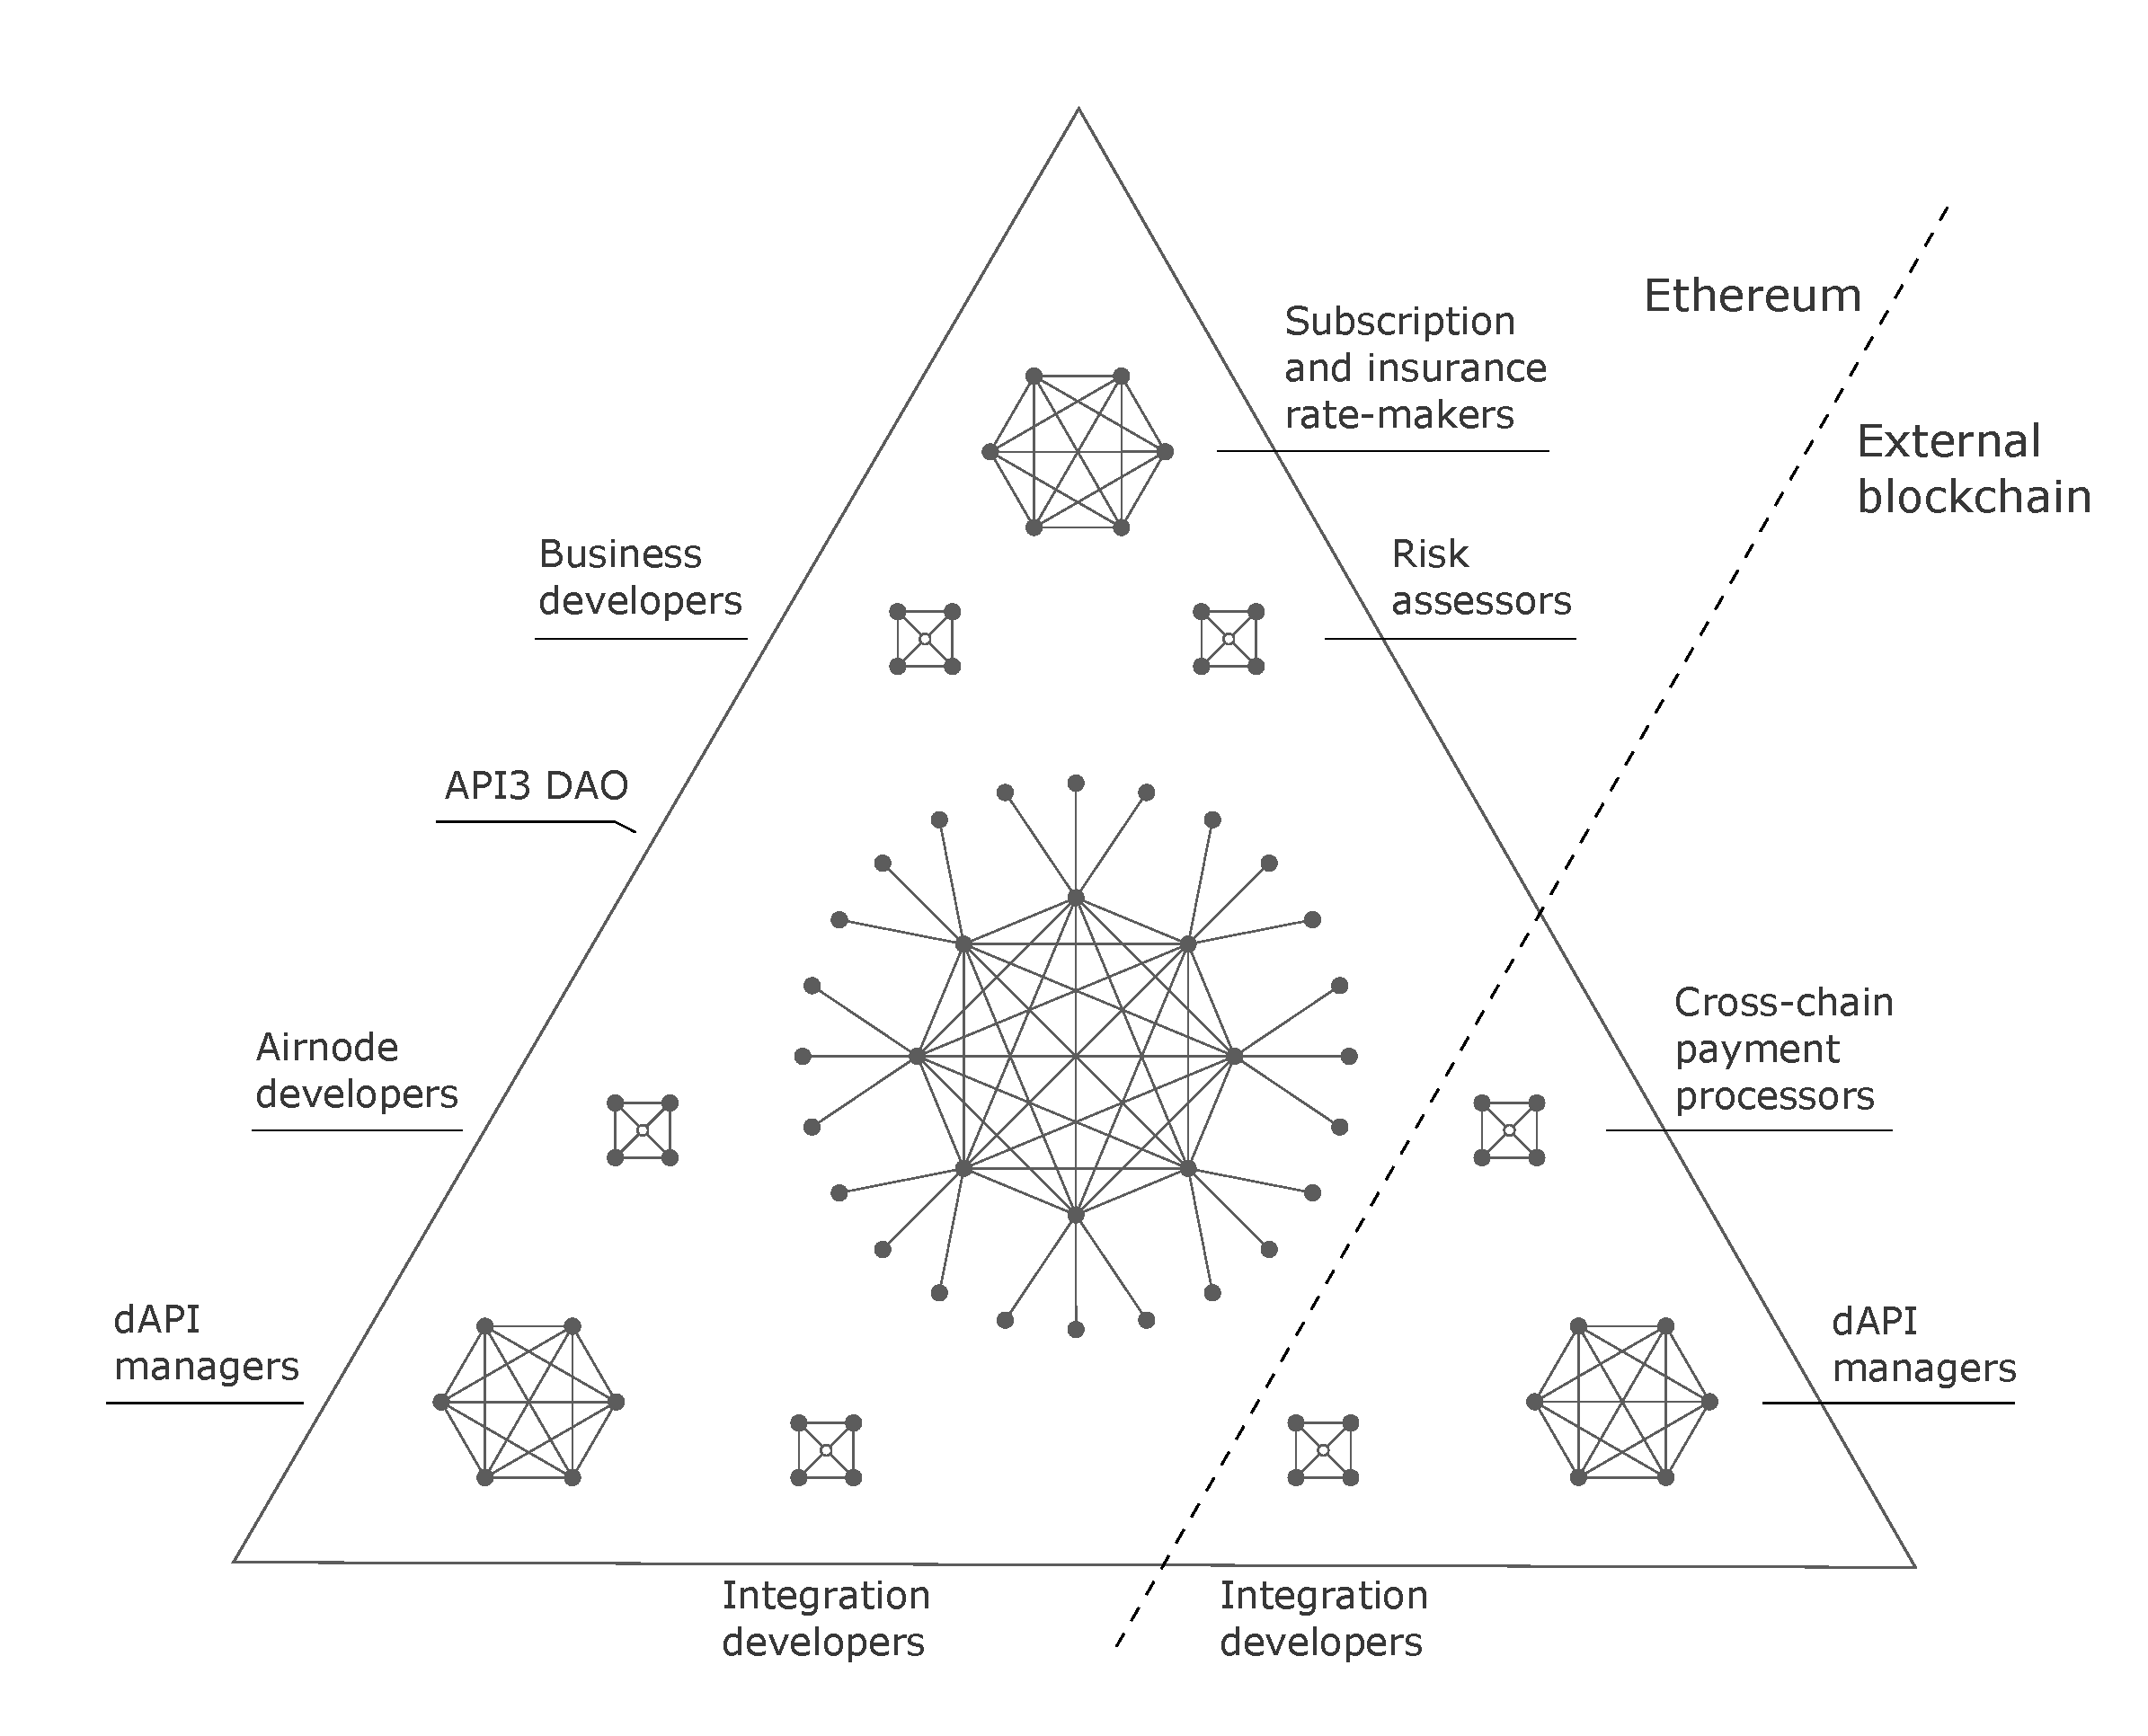
\includegraphics[width=\textwidth]{fig/dao.pdf}
	\caption{Un ejemplo de estructura jerárquica de gobierno, compuesta por el DAO principal, los subDAOs y los equipos distribuidos a través de cadenas. El DAO principal gobierna asignando selectivamente fondos y delegando la autoridad. Cuando una tarea alcanza una escala que ya no puede ser cumplida por un equipo, es asignado a un subDAO.}
	\label{fig:dao}
\end{figure}

Este esquema de gobierno basado en equipos es escalable en términos de costos del gas, ya que requiere menos propuestas para ser votadas a nivel del DAO. También es más escalable en términos prácticos, ya que no requiere la atención constante de todas las partes gobernantes a una amplia variedad de detalles minuciosos. Además, permite que operaciones críticas como la gestión de la dAPI se ejecuten rápidamente y se basen en la opinión de los expertos. A medida que las operaciones del API3 se vayan ampliando, esta jerarquía de gobierno puede exigir capas adicionales, lo que implica subDAOs (véase la Figura~\ref{fig:dao}).

El DAO debe seguir dos principios para que este esquema sea efectivo. En primer lugar, para limitar la cantidad de daños que puede causar un equipo malintencionado o incompetente, la autoridad de la que dispone el equipo debe limitarse al mínimo, lo que también se conoce como el "principio del mínimo privilegio". Por ejemplo, un equipo de gestión de una dAPI nunca debe poder recomponer completamente una dAPI que esté en uso, sino que sólo debe ser capaz de cambiar los oráculos individuales dentro y fuera con un período de reposo lo suficientemente largo como para asegurar que no se pueda abusar de su autoridad en un grado significativo. Del mismo modo, los hitos y los resultados deben utilizarse para conceder a los equipos sólo los fondos que necesiten para cumplir las responsabilidades específicas que tengan en ese momento. El segundo principio es la transparencia. Para que el DAO pueda evaluar su desempeño, el equipo debe informar a el DAO de manera muy detallada. Estos informes tendrán la ventaja adicional de proporcionar una rendición de cuentas y permitirán a los usuarios de la dAPI y al público en general poder auditar las operaciones de la API3 en todo momento. 

\subsection{Monetización de dAPI y compensación del proveedor de API}
\label{sec:dapi-monetization-and-api-provider-compensation}

Las cuotas de suscripción a la API suelen pagarse mensual o anualmente, ya que este plan se adapta tanto a los proveedores de API como a sus clientes. El objetivo de la API3 será seguir el mismo esquema para las dAPIs. Para acceder a una dAPI, el usuario pagará una cuota de suscripción recurrente, que puede ser fija o personalizada para el usuario en función de su caso de uso particular. Estos precios serán determinados por el equipo respectivo, e incluirán la prima si el usuario desea recibir el servicio de seguro descrito en la Sección~\ref{sec:quantifiable-security-through-insurance}.
El pago podrá efectuarse en cualquier criptomoneda, que será recibida por el DAO en tokens API3 a través de una casa de cambio descentralizada basada en un fondo común de liquidez.

Los proveedores de API serán compensados periódicamente a tasas fijas, que se ajustarán a sus modelos de precios actuales. Esto se hará utilizando stablecoins siempre que sea posible, aunque, como se menciona en la Sección~\ref{sec:barriers-to-api-providers-operating-oracles}, algunos proveedores de API rechazan categóricamente el manejo de la criptomoneda como pago. En tales casos, el DAO proporcionará un subsidio que se pagará a cambio de la prueba que el proveedor de la API sea compensado en fiat por el beneficiario.

\subsection{dAPIs Multiplataforma}
\label{sec:cross-platform-dapis}

La API3 utilizará xDai~\cite{xdai:2019} como solución de escalado de segunda capa, por lo que trabajar de forma multiplataforma será una parte ordinaria de sus operaciones. El mismo flujo de trabajo que se desarrollará para unir xDai con Ethereum se utilizará para unirlo con otras plataformas de contratos inteligentes, lo que permitirá a la API3 servir dAPIs multiplataforma. Estas integraciones entre plataformas se llevarán a cabo y se mantendrán mediante subsidios, que se concederán a equipos compuestos parcialmente por miembros de los respectivos ecosistemas de las plataformas de contratos inteligentes.

Hemos descrito un esquema para compensar a los proveedores de API en moneda fiat en la Sección~\ref{sec:dapi-monetization-and-api-provider-compensation}.
En lo que respecta a las cuotas de suscripción a la dAPI multiplataforma, necesitamos que el DAO API3 sea compensada a través de las plataformas de contratos inteligentes, lo que constituye un problema similar.
 
Por lo tanto, utilizaremos un análogo de la misma solución, en el que un beneficiario pagará al DAO API3 a cambio de estar autorizado a recibir pagos en su nombre en otra plataforma de contratos inteligentes. Por ejemplo, si el DAO necesita que se le paguen 100 tokens API3 como cuota de suscripción, el beneficiario pagará 90 tokens API3 al DAO, lo que dará lugar a que se entienda que el beneficiario está autorizado a recibir el pago de 100 tokens API3 en nombre de otra cadena. Este proceso se formalizará según se requiera.

Mediante la aplicación del puente de datos y el canal de pago, la API3 podrá prestar servicio a otras plataformas de contratos inteligentes sin necesidad de que interactúen con el Ethereum o manejen los tokens de la API3. Obsérvese que el Ethereum se utilizará como capa de resolución de disputas para el servicio de seguros descrito en la Sección~\ref{sec:quantifiable-security-through-insurance} hasta que surja una alternativa multiplataforma.

\subsection{Tokenomics API3 \footnote{See the link for the update \url{https://medium.com/api3/api3-tokenomics-update-f032d6e49b30}}}
\label{sec:api3-tokenomics}

La gobernanza descentralizada requiere mecanismos de incentivo bien equilibrados que modelen con precisión los resultados tanto positivos como negativos. En otras palabras, las entidades rectoras deben ser recompensadas por los buenos resultados y penalizadas por los malos. El token API3 está diseñado para facilitar esto a través de tres utilidades principales:

\begin{enumerate}
    \item Apilamiento: Otorga ingresos de la dAPI y recompensas inflacionarias.
    \item Garantía: Respalda los servicios de seguro que protegen a los usuarios de los daños causados por el mal funcionamiento de la dAPI.
    \item Gobernanza: Otorga representación directa en el DAO API3.
\end{enumerate}

El servicio de apilamiento proporciona un incentivo financiero para participar en la API3 y contribuir a aumentar sus ingresos. La utilidad de la garantía hace que los participantes compartan el riesgo operacional de la API3 y los incentiva para minimizarlo. Por último, la utilidad de gobernanza ofrece a los participantes el instrumento definitivo para promulgar esos incentivos.

Obsérvese que es fundamental que estas tres utilidades coincidan. Todas las entidades rectoras deben recibir recompensas de apilamiento para que gobiernen de manera que se maximicen los ingresos. Todas las entidades rectoras deben utilizar sus fondos como garantía para que gobiernen de manera que se minimicen los riesgos de seguridad. A tal fin, la API3 tendrá un fondo común de apilamiento. Al apilar tokens API3 en este fondo común, se concederá representación y recompensas de apilamiento, pero al mismo tiempo, los tokens apilados se utilizarán como garantía para pagar las indemnizaciones de seguros según sea necesario.

\subsubsection{Apilamiento}
\label{sec:staking}

La API3 tiene como objetivo establecer, mantener y monetizar las dAPIs a escala. Su éxito al hacerlo puede estimarse por sus ingresos totales, ya que éstos aumentarán con el número de dAPI y la cantidad de fondos que obtengan. Para alinear los incentivos de gobernanza con el éxito de la API3, una parte de estos ingresos decididos por el DAO se distribuirá a los apiladores.  Se espera que este mecanismo domine los incentivos positivos de apilamiento a medida que la API3 gane tracción.

Las recompensas de apilamiento inflacionario son un mecanismo comprobado en la práctica que resulta útil para iniciar y mantener un fondo común que necesita colateralizar en exceso un servicio ~\cite{synthetix:2020}, por ejemplo, el servicio de seguro dAPI que se describe en la Sección~\ref{sec:quantifiable-security-through-insurance}.
También es una buena herramienta de distribución de tokens que favorece a los poseedores que participan en el sistema sobre los pasivos. Por lo tanto, las recompensas inflacionarias se utilizarán para incentivar aún más el apilamiento.

\begin{figure}[t]
     \centering
     \begin{subfigure}{0.9\textwidth}
         \centering
         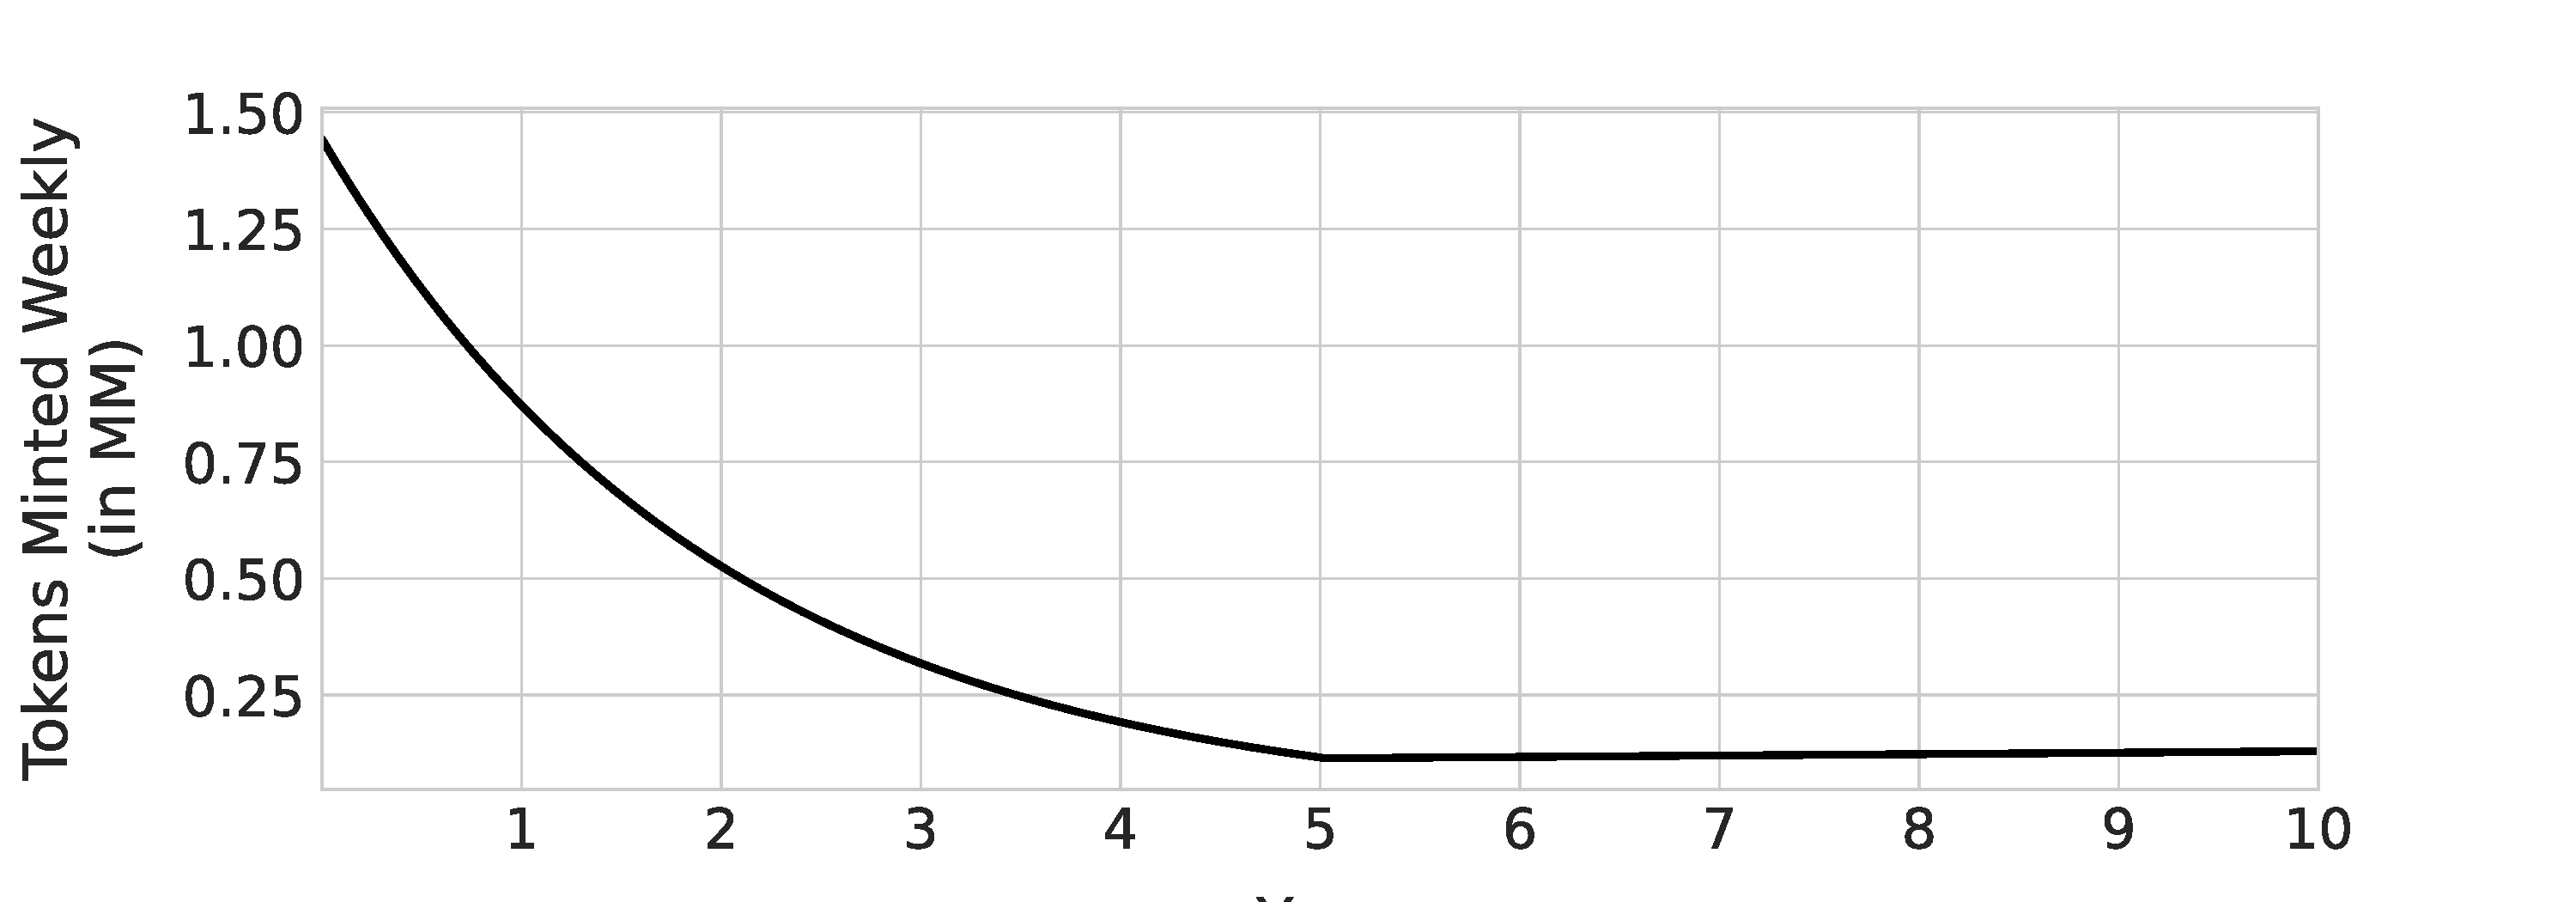
\includegraphics[width=\textwidth]{fig/token-weekly-emission.pdf}
         \caption{El número de tokens emitidos cada semana se reduce exponencialmente para disminuir la tasa de inflación anual del  $75\%$ al $2.5\%$ hasta el final del quinto año. Al final de ese año, la tasa de inflación anual se fija en un $2.5\%$ constante.}
         \label{fig:token-emission}
     \end{subfigure}
     \begin{subfigure}{0.9\textwidth}
         \centering
         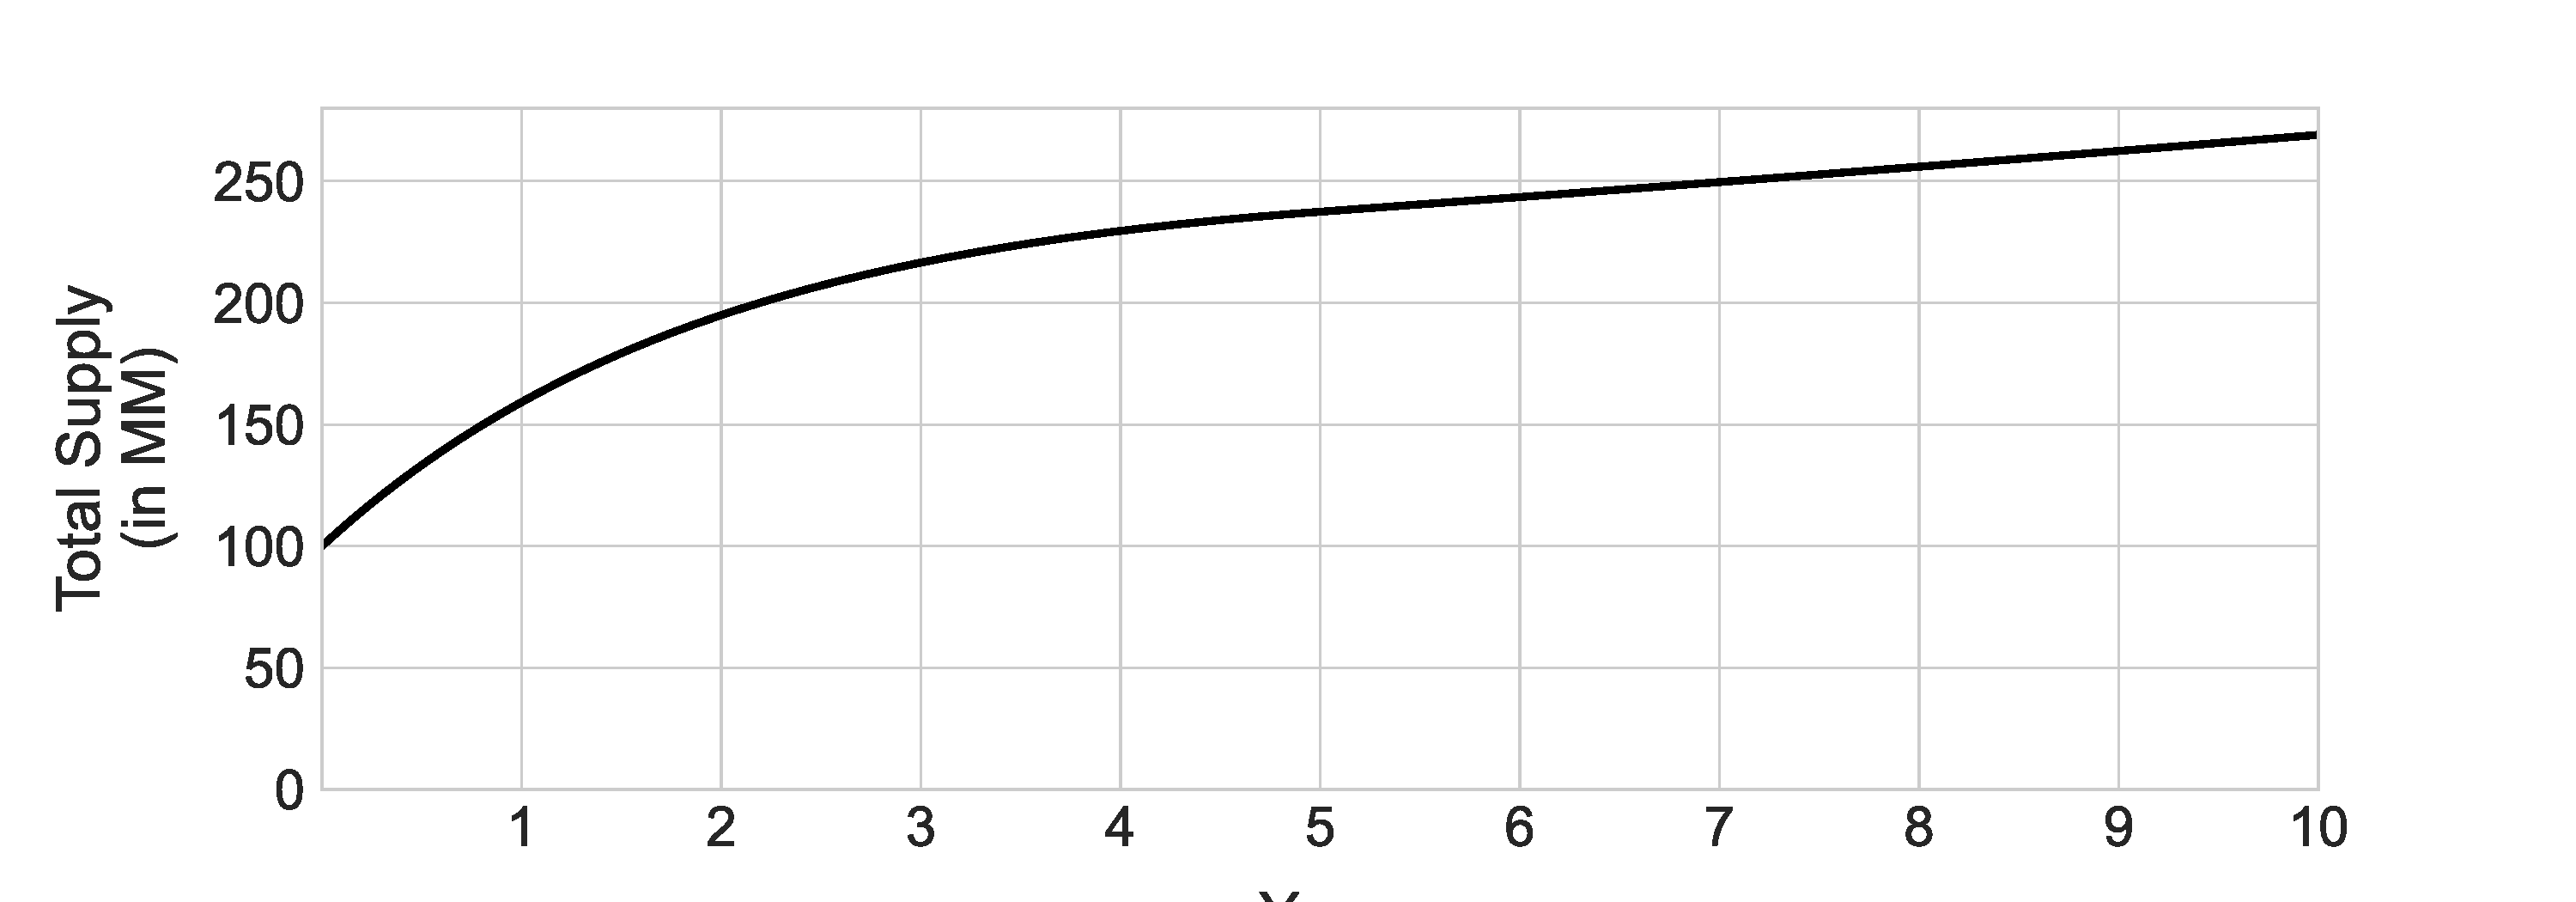
\includegraphics[width=\textwidth]{fig/token-total-supply.pdf}
         \caption{El suministro total de tokens para la API3 comienza a partir de 100 millones y aumenta de acuerdo con la planificación que se indica en (a).}
         \label{fig:total-supply}
     \end{subfigure}
    \caption{Programa de inflación de tokens API3 para recompensas de apilamiento.}
    \label{fig:token}
\end{figure}

En esencia, las recompensas inflacionarias obligan a los poseedores de tokens a apilar para preservar el valor de sus tokens. Sin embargo, el hecho de apilar es arriesgado debido a que los fondos se utilizan como garantía, y obliga al apilador a participar en la gobernanza para asegurar que el riesgo se reduzca al mínimo (un mecanismo similar se propone recientemente en~\cite{aave}).
Como combinación de ambos, una token de gobernanza inflacionaria utilizada como garantía obliga a todos los poseedores de tokens a participar en la gobernanza, lo que resulta ideal porque maximiza la descentralización de la misma. Además, las recompensas inflacionarias se conceden durante un año, lo que da lugar a que los partidos gobernantes compartan los intereses a largo plazo del proyecto.

Las recompensas inflacionarias comenzarán a una tasa anual del  75\% (1.44\% semanal), y el número de tokens emitidos semanalmente se reducirá exponencialmente hasta que la tasa de inflación anual se convierta en el  2.5\% al final del quinto año. A partir de este momento, la inflación anual se mantendrá en una tasa del 2.5\% a perpetuidad (véase la Figura e~\ref{fig:token-emission}).
El cambio en la oferta total de tokens API3 se ilustra en la Figura~\ref{fig:total-supply}.
El esquema de inflación propuesto se adapta de\cite{sip-24} y será gobernable.

\subsubsection{Garantia}
\label{sec:collateral}

Si apilar en la API3 sólo reportara recompensas, el único incentivo de gobierno sería maximizar los ingresos. Esto se haría aumentando agresivamente el número de usuarios de dAPI y la cantidad que se garantiza con ellos. En la Sección ~\ref{sec:middleman-tax}, hemos demostrado que la carga total a la que está sometida una dAPI aumenta la probabilidad de que falle debido a un ataque. Por lo tanto, esta no es una estrategia de gobierno sostenible para la alimentación descentralizada de datos.

Exponer a las partes gobernantes al riesgo que estamos tratando de evitar alinearía sus incentivos con los de los DAO. Entonces, los partidos gobernantes deben ser penalizados cuando se produce un fallo de la dAPI. Fuimos un paso más allá y diseñamos un servicio de seguro on-chain que proporciona a los usuarios de dAPI garantías de seguridad cuantificables y de confianza. Este servicio de seguro utiliza como garantía el fondo de apilamiento con tokens API3, lo que significa que cuando se confirma un fallo de dAPI a través del protocolo de resolución de disputas, los daños del usuario serán cubiertos por el fondo de apilamiento. Véase la Sección \ref{sec:quantifiable-security-through-insurance} para los detalles de cómo se implementará este servicio de seguro. 

\begin{figure}
     \centering
     \begin{subfigure}{0.49\textwidth}
         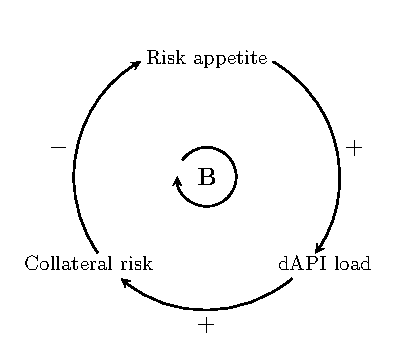
\includegraphics[width=\textwidth]{fig/systems-diagram.pdf}
         \caption{Diagrama de sistemas de gobernanza}
         \label{fig:systems-diagram}
     \end{subfigure}
     \begin{subfigure}{0.49\textwidth}
         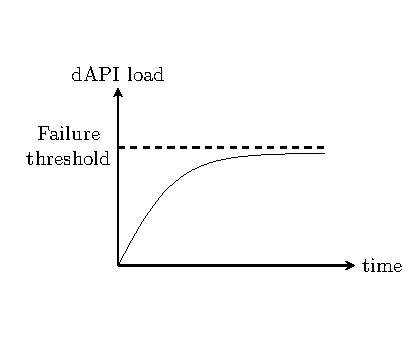
\includegraphics[width=\textwidth]{fig/systems-diagram-plot.pdf}
         \caption{Carga de dAPI a lo largo del tiempo en un sistema equilibrado}
         \label{fig:systems-diagram-plot}
     \end{subfigure}
    \caption{Las utilidades de apilamiento y de garantía de seguro del token API3 dan lugar a incentivos de gobierno equilibrados. 
    \textbf{(a)} La carga de las dAPIs con más usuarios aumenta la probabilidad de que se paguen las reclamaciones de seguro, lo que produce una retroalimentación negativa y equilibra el sistema.
   \textbf{(b)} Debido al carácter equilibrado del sistema, la carga de dAPI no aumenta indefinidamente, sino que se establece a un nivel que el DAO estima que es inferior a la carga máxima que pueden soportar las dAPIs.}
    \label{fig:systems-diagram-full}
\end{figure}

Veamos el efecto de la utilización del fondo común de apilamiento tanto para la garantía como para la gestión en un diagrama de sistemas de la Figura ~\ref{fig:systems-diagram}.
Cuando el DAO tiene apetito de riesgo adicional, se incorpora a nuevos usuarios de dAPI, lo que aumenta su carga de trabajo. Esto aumenta la probabilidad de un fallo de la dAPI, la probabilidad de pagar una reclamación de seguro y el riesgo colateral global resultante.  Con el aumento del riesgo colateral, se suprime el apetito de riesgo del DAO. En otras palabras, la retroalimentación negativa causada por el servicio de seguros impide el crecimiento autodestructivo. Véase la Figura ~\ref{fig:systems-diagram-plot} para el comportamiento esperado de la carga de dAPI que surgirá de esto. El DAO estima un umbral de fallo para las dAPIs, y los usuarios a bordo convergen a este valor, pero no lo supera. Obsérvese que en el caso de que el DAO sobreestime este umbral, las dAPIs no funcionarán y las partes gobernantes serán castigadas, ya que sus fondos apilados se utilizarán para pagar la reclamación de seguro hecha por los usuarios de dAPI afectados. En otras palabras, los usuarios de la dAPI están protegidos en ambos casos.

\subsubsection{Gobernanza}
\label{sec:governance}

La única manera de obtener representación en el DAO API3 será apilando tokens de la API3 en el fondo común de garantía de seguros. De este modo, las partes gobernantes estarán expuestas a todos los riesgos y recompensas del API3, y gobernarán para optimizarlos.

Las recompensas inflacionarias y los tokens de gobernanza apilados que se utilicen como garantía crearán un circuito de retroalimentación positiva en términos de calidad de la gobernanza. Los titulares de los tokens iniciales tendrán que apilar y exponerse al riesgo si no quieren perder valor ante la inflación. Si se equivocan en el gobierno y pierden la garantía mediante reclamaciones de seguros, estas fichas serán devueltas al mercado abierto, desde donde serán adquiridas por los nuevos partidos gobernantes. Por el contrario, si los titulares de los tokens iniciales gobiernan bien y causan escasez de tokens en el mercado, la distribución de la representación estará protegida. En otras palabras, los tokens de gobierno que se utilizan como garantía dan lugar a una robusta estructura Darwiniana que se mejora a sí misma y es capaz de recuperarse de los fracasos.


%~~~~~~~~~~~~~~~~~~~~~~~~~~~~~~~~~~~~~~~~~~~~~~~~~~~~~~~~~~~~~~~~~~~

\section{Seguridad Cuantificable a través del Seguro}
\label{sec:quantifiable-security-through-insurance}

La API3 proporcionará a los usuarios de la dAPI un nivel de seguridad cuantificable en forma de un servicio de seguro on-chain. Esto logra dos objetivos: (1) el seguro actúa como una red de seguridad bien definida y de confianza para el usuario en caso de un fallo en el sistema de seguridad; (2) hace responsables a los gobernantes de los fallos de la dAPI, y por lo tanto los incentiva a gobernar hacia dAPIs más seguros.

\subsection{La necesidad por seguridad cuantificable}
\label{sec:the-need-for-quantifiable-security}

\begin{quote}
\it
La ingeniería es el arte de modelar materiales que no comprendemos del todo, en formas que no podemos analizar con precisión, para soportar fuerzas que no podemos evaluar adecuadamente, de tal manera que el público no tiene motivos para sospechar el alcance de nuestra ignorancia.
\end{quote}
\begin{flushright}
-- Dr. A. R. Dykes
\end{flushright}

Si le preguntáramos a un ingeniero "¿Cuánta carga puede soportar su puente?" y obtuviéramos la respuesta "Puedo asegurarle que tiene 21 vigas de acero de la más alta calidad", no querríamos usar ese puente, ya que, no ser capaz de proporcionar la máxima carga es una señal de alerta de la ingeniería. Hemos introducido un modelo simplista de cuánto sería capaz de soportar un solo oráculo y, por consecuencia, una alimentación de datos en la Sección~\ref{sec:middleman-tax}.
Aunque no es exhaustivo, este modelo demuestra que las redes descentralizadas de oráculos no pueden asegurar un valor monetario arbitrariamente grande. La cantidad asegurada por un oráculo debe ser limitada. En otras palabras, como toda la tecnología de la cadena de bloques, las redes de oráculos descentralizadas sólo deben ser confiadas hasta cierto punto, en lugar de ser tratadas como incondicionalmente desconfiables~\cite{defilippi:2020}.
Entonces, un alimentador de datos —centralizado~\cite{coinbase} o descentralizado~\cite{ellis:2017}---debería encargarse de cuantificar la cantidad que puede asegurar.

Una de las más reconocidas soluciones a este problema se propone para el protocolo UMA ~\cite{uma:2020}.
El esquema propuesto no sólo permite la cuantificación de la cantidad que puede asegurarse mediante una alimentación de datos utilizando principios de teoría de juegos, sino que también permite establecer con precisión este límite. Los autores observan astutamente que un suministro de datos demasiado seguro no es deseable porque será innecesariamente costoso para sus usuarios, y el hecho de poder fijar el grado de seguridad en los requisitos mínimos reduciría los costos. Sin embargo, siguen con la afirmación de que el método que han propuesto es óptimo en cuanto a la rentabilidad, lo cual es sumamente inexacto en la práctica. Este error se debe a que se aborda el problema de forma ciega a la fuente de datos, es decir, tratando de resolver el problema del oráculo en lugar del problema de la conectividad de la API. La solución propuesta sólo es óptima si consideramos que todos los oráculos son poco fiables, lo que constituye una aproximación suficientemente cercana para los oráculos de terceros. En cambio, la fiabilidad de los oráculos de primera mano puede aprovecharse para crear fuentes de datos extremadamente seguras a un costo muy bajo, ya que los proveedores de la API tienen demasiado que perder al intentar un ataque. Que un producto DeFi de alto valor esté asegurado con éxito por los datos proporcionados por un único intercambio centralizado de buena reputación demuestra muy bien este hecho~\cite{coinbase}.
Por lo tanto, no se puede esperar que se pase por alto la fiabilidad demostrada y se acabe con una solución realmente rentable.

La solución ideal que se ajuste a la visión de la API3 debe proporcionar garantías de seguridad cuantificables aprovechando la fiabilidad de los proveedores de API, que sólo puede evaluarse utilizando información off-chain. Para ello, la API3 proporcionará un servicio de seguro que garantice a un usuario de la dAPI que los daños debidos a un fallo estarán cubiertos hasta un monto predeterminado. Esta solución es preferible para el usuario, ya que una solución alternativa de la teoría de juegos puede fallar inesperadamente debido a incentivos mal modelados o no contabilizados.

\subsection{Seguro dAPI}
\label{sec:dapi-insurance}

En la Sección~\ref{sec:centralized-oracle-network-governance}, mencionamos un incidente de seguridad en el que un alimentador de datos Chainlink había informado erróneamente a Synthetix. Se informó que esto causó daños menores a 40,000 dólares para Chainlink el día del incidente ~\cite{chainlink-fatfinger} y aproximadamente 36.000 dólares para Synthetix el día después ~\cite{synthetix-fatfinger}.
Además, Synthetix anunció que Chainlink había ofrecido compensar los daños, lo que posteriormente aceptó. Este incidente ha demostrado lo siguiente:

\begin{enumerate}
    \item El seguro que paga los daños es una solución natural y obvia para el fallo de la alimentación de datos.
    \item Se entiende generalmente que la entidad gobernante es responsable de fallos en la alimentación de datos.
    \item Es posible determinar los fallos de alimentación de datos, sus causas y los daños resultantes en cuestión de días.
\end{enumerate}

A primera vista, este incidente se resolvió sin problemas. Esto es de esperar, ya que la cantidad en cuestión era relativamente insignificante para las respectivas partes. Sin embargo, ni el público en general ni las partes interesadas pueden estar seguros de los términos exactos ya que ambos proyectos se rigen de forma centralizada. Esto nos lleva para preguntar: ¿Qué habría pasado si los daños fueran de una magnitud mayor? ¿Cómo se supone que los proyectos totalmente descentralizados deben hacer frente a tales eventos?

Se ha demostrado que el uso de los seguros no sólo se correlaciona con el crecimiento macroeconómico, sino que también es una causa del mismo ~\cite{outreville:2013}.
Sin embargo, los seguros están muy infrautilizados en el espacio de la cadena de bloques. Una de las principales razones de esto es que el seguro requiere naturalmente de un tercero para resolver las disputas, y utilizar un tercero de confianza mutua para este propósito va en contra de la ética de la descentralización. Sin embargo, el surgimiento de Kleros ~\cite{kleros:2019}, un protocolo de propósito general para la resolución de disputas on-chain, permite construir productos de seguros sin necesidad de confianza.

La API3 desarrollará conjuntamente con Kleros un servicio de seguros on-chain que proporcione garantías de seguridad cuantificables y sin necesidad de confianza Este servicio de seguro protegerá al usuario de dAPI contra los daños causados por ciertos fallos de dAPI hasta un límite de reembolso. Obsérvese que incluso si no proporcionáramos este servicio, el usuario de la dAPI podría haber recibido servicios de seguro on-chain utilizando una solución de terceros~\cite{nexus-mutual}.
Esa solución tendería a cobrar primas de seguro muy elevadas, ya que no tendrían acceso a la información y los conocimientos técnicos necesarios para evaluar con precisión los riesgos de la dAPI. Además, como se describe en la Sección ~\ref{sec:collateral}, el servicio de seguro propuesto es especial por la forma en que está garantizado por los fondos aportados por los partidos gobernantes del DAO API3. Por lo tanto, no sólo proporciona garantías de seguridad al usuario de los dAPI, sino que también crea un fuerte incentivo para que los dAPIs se rijan de manera que se maximice su seguridad, lo que reducirá aún más los costos del seguro.

\subsection{Proceso de seguro}
\label{sec:insurance-process}

El usuario solicita suscribirse a una dAPI y recibir una cobertura de seguro específica para el servicio respectivo a través de canales off-chain. La cantidad total que puede cubrirse está limitada por el tamaño del fondo común de garantías, y el DAO regirá el coeficiente de garantía basado en la literatura existente sobre solvencia de los seguros ~\cite{solvency}.
Los respectivos equipos de la API3 investigan los riesgos de fallos de la DAPI y el caso de uso específico del usuario, calculan la prima de seguro e introducen la cuota específica del usuario en el contrato que gestiona los pagos.  Al pagar la cuota al contrato, el usuario tiene acceso al dAPI y se asegura para el período de pago respectivo.

Si el usuario de la dAPI nota un mal funcionamiento, evaluará los daños y hará una reclamación al seguro on-chain. Esto bloqueará automáticamente la cantidad reclamada en el fondo común de garantía descrito en la Sección ~\ref{sec:api3-tokenomics}.
Los retiros de las participaciones tendrán un plazo adecuado que evitará que los titulares de las mismas presenten reclamaciones por adelantado, es decir, que se retiren tan pronto como la dAPI falle para evadir reclamos. Por otro lado, el asegurado necesitará apilar fondos para poder hacer un reclamo para desincentivar el abuso. El DAO API3 puede pagar el reclamo directamente o elevarla al tribunal de Kleros, que determinará si la cantidad reclamada se pagará al usuario de la dAPI. Si se rechaza la reclamación, se desbloquearán los tokens, mientras que, si se acepta, los tokens se transferirán al usuario de la dAPI. Esto corresponde a los apiladores que cubren los daños proporcionales a la cantidad que han apilado; es decir, un usuario que ha apilado tokens que constituyen el $p\%$ de todo el fondo común pagará el $p\%$ de una reclamación aceptada.

El esquema descrito anteriormente supone que todas las cantidades se denominarán en tokens API3. Dependiendo del caso, algunos usuarios pueden requerir estar asegurados en otros tipos de criptomonedas, por ejemplo, ETH. En este caso, no bastará con que un proveedor de liquidez convierta automáticamente el pago a ETH, ya que la tasa de cambio API3/ETH, entre el momento en que se hace el reclamo y se paga, cambiará, lo que dará lugar a un desfase. Como solución, el DAO API3 puede mantener una reserva adicional de ETH —sujeto a las mismas consideraciones de solvencia que el fondo común de garantías— para absorber la volatilidad de los precios y asegurar que el pago se ajuste al monto que el usuario ha reclamado originalmente..

\subsection{Evaluación de riesgos}
\label{sec:risk-assessment}

Cuantificar el grado de seguridad que puede proporcionar una alimentación de datos es un problema muy difícil. Sin embargo, al integrar el problema en el dominio de los seguros establecidos, se obtiene acceso a una amplia variedad de literatura y conocimientos que se pueden obtener fácilmente de los servicios de seguros tradicionales. Por lo tanto, la API3 estará bien equipada con los servicios de actuarios, estadísticos, científicos de datos, tarificadores, analistas y asesores jurídicos para asumir la difícil tarea de proporcionar garantías de seguridad cuantificables.

La evaluación de riesgos es un paso vital para optimizar la fijación de precios de los seguros y hacer estimaciones correctas de la solvencia. Esto incluye dos factores principales:

\begin{itemize}
    \item Interno: ¿Qué probabilidad hay de que la dAPI falle?
    \item Externo: ¿Cuál es el valor esperado de los daños causados por un posible mal funcionamiento de la dAPI?
\end{itemize}

Uno de los factores de riesgo interno más importantes en este caso es el fracaso al nivel del oráculo, que puede ser estimado investigando cualitativamente las APIs individuales y analizando su rendimiento estadísticamente. Por ejemplo, las investigaciones cualitativas pueden llegar a la conclusión de que un proveedor de API ha estado en el negocio durante 5 años, y por lo tanto no constituye un riesgo significativo de ataque Sybil. Análogamente, el análisis estadístico puede indicar que los datos proporcionados por un proveedor de API suelen divergir del consenso, lo que puede plantear un problema si el consumidor de los datos exige una gran precisión. Esas evaluaciones también servirán de orientación para elaborar dAPIs en lo que respecta al número y la selección de los proveedores de API, por ejemplo, puede comprobarse que si se añaden más APIs a una dAPI sobrecargada se terminará reduciendo los costos al disminuir el riesgo de seguro. Los riesgos operacionales son otro factor importante, que puede evaluarse mediante auditorías que investiguen los procesos operacionales. Obsérvese que, dado que esta investigación será realizada por los equipos de la API3 y se informará públicamente a el DAO, proporcionará a los usuarios una transparencia y una garantía de seguridad inigualables.

\begin{figure}[!t]
     \centering
     \begin{subfigure}{0.38\textwidth}
         \centering
         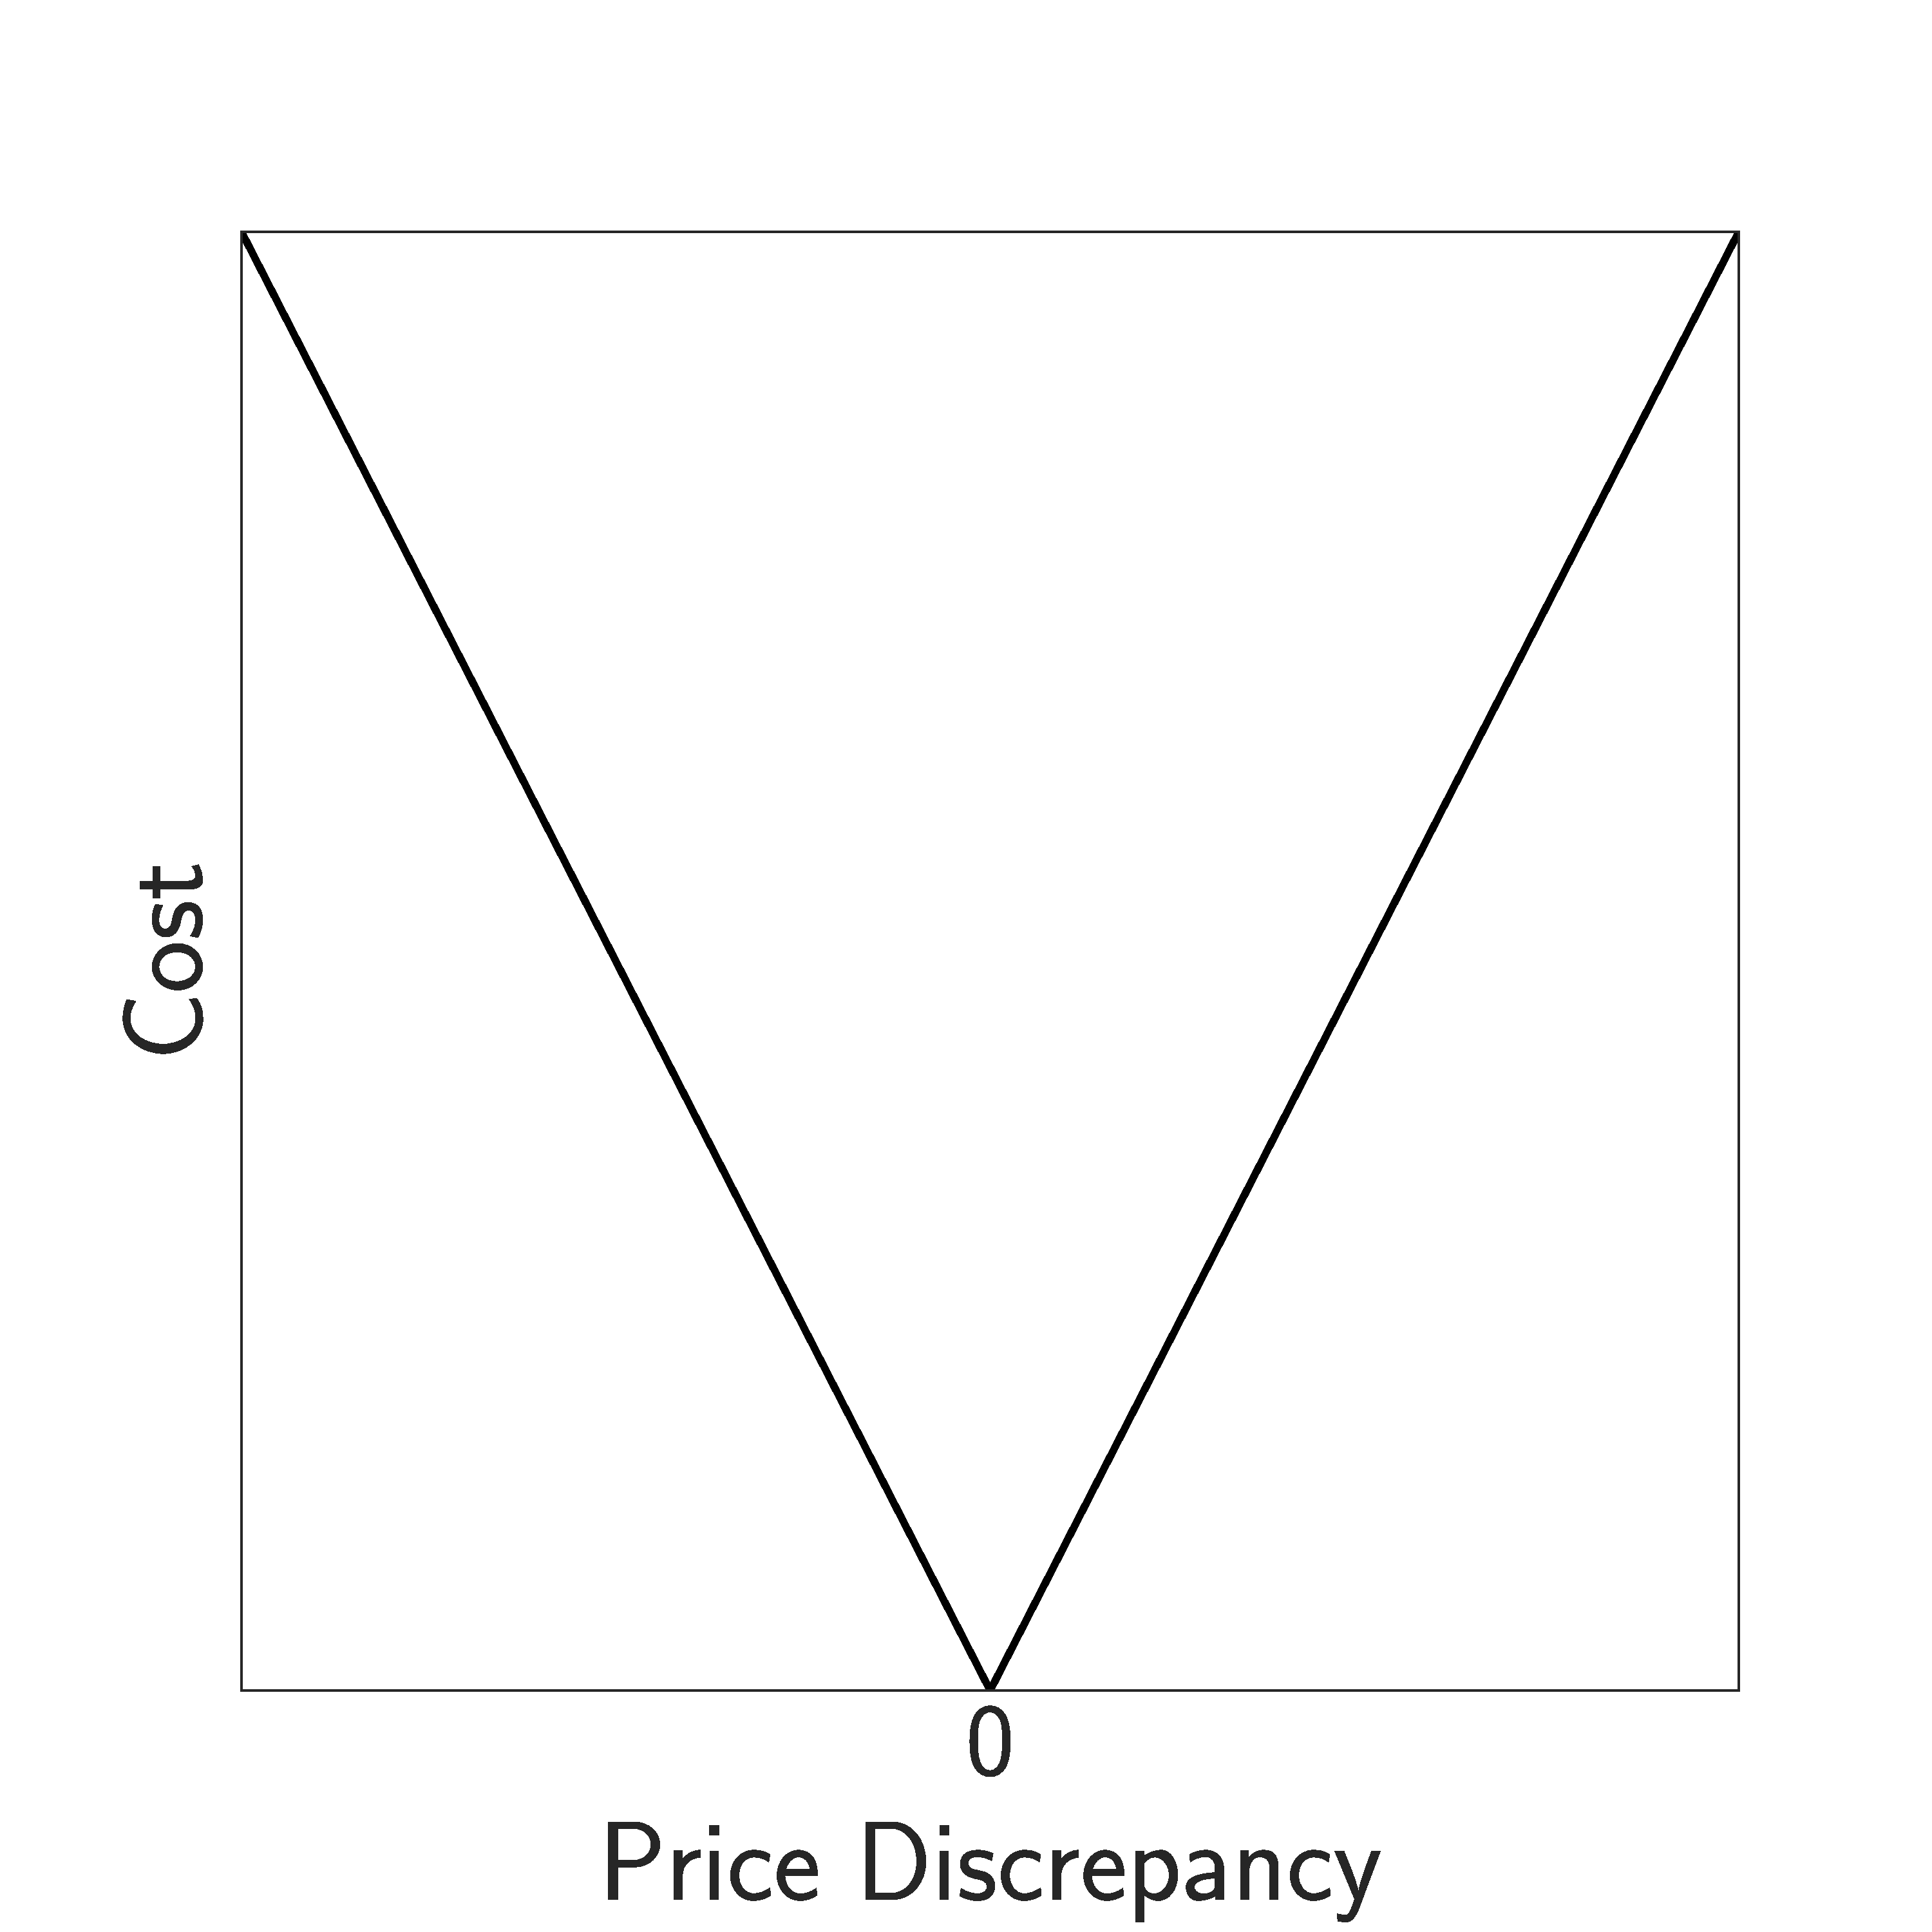
\includegraphics[width=\textwidth]{fig/use-case-linear.pdf}
         \caption{linear}
         \label{fig:use-case-linear}
     \end{subfigure}
     
     \begin{subfigure}{0.38\textwidth}
         \centering
         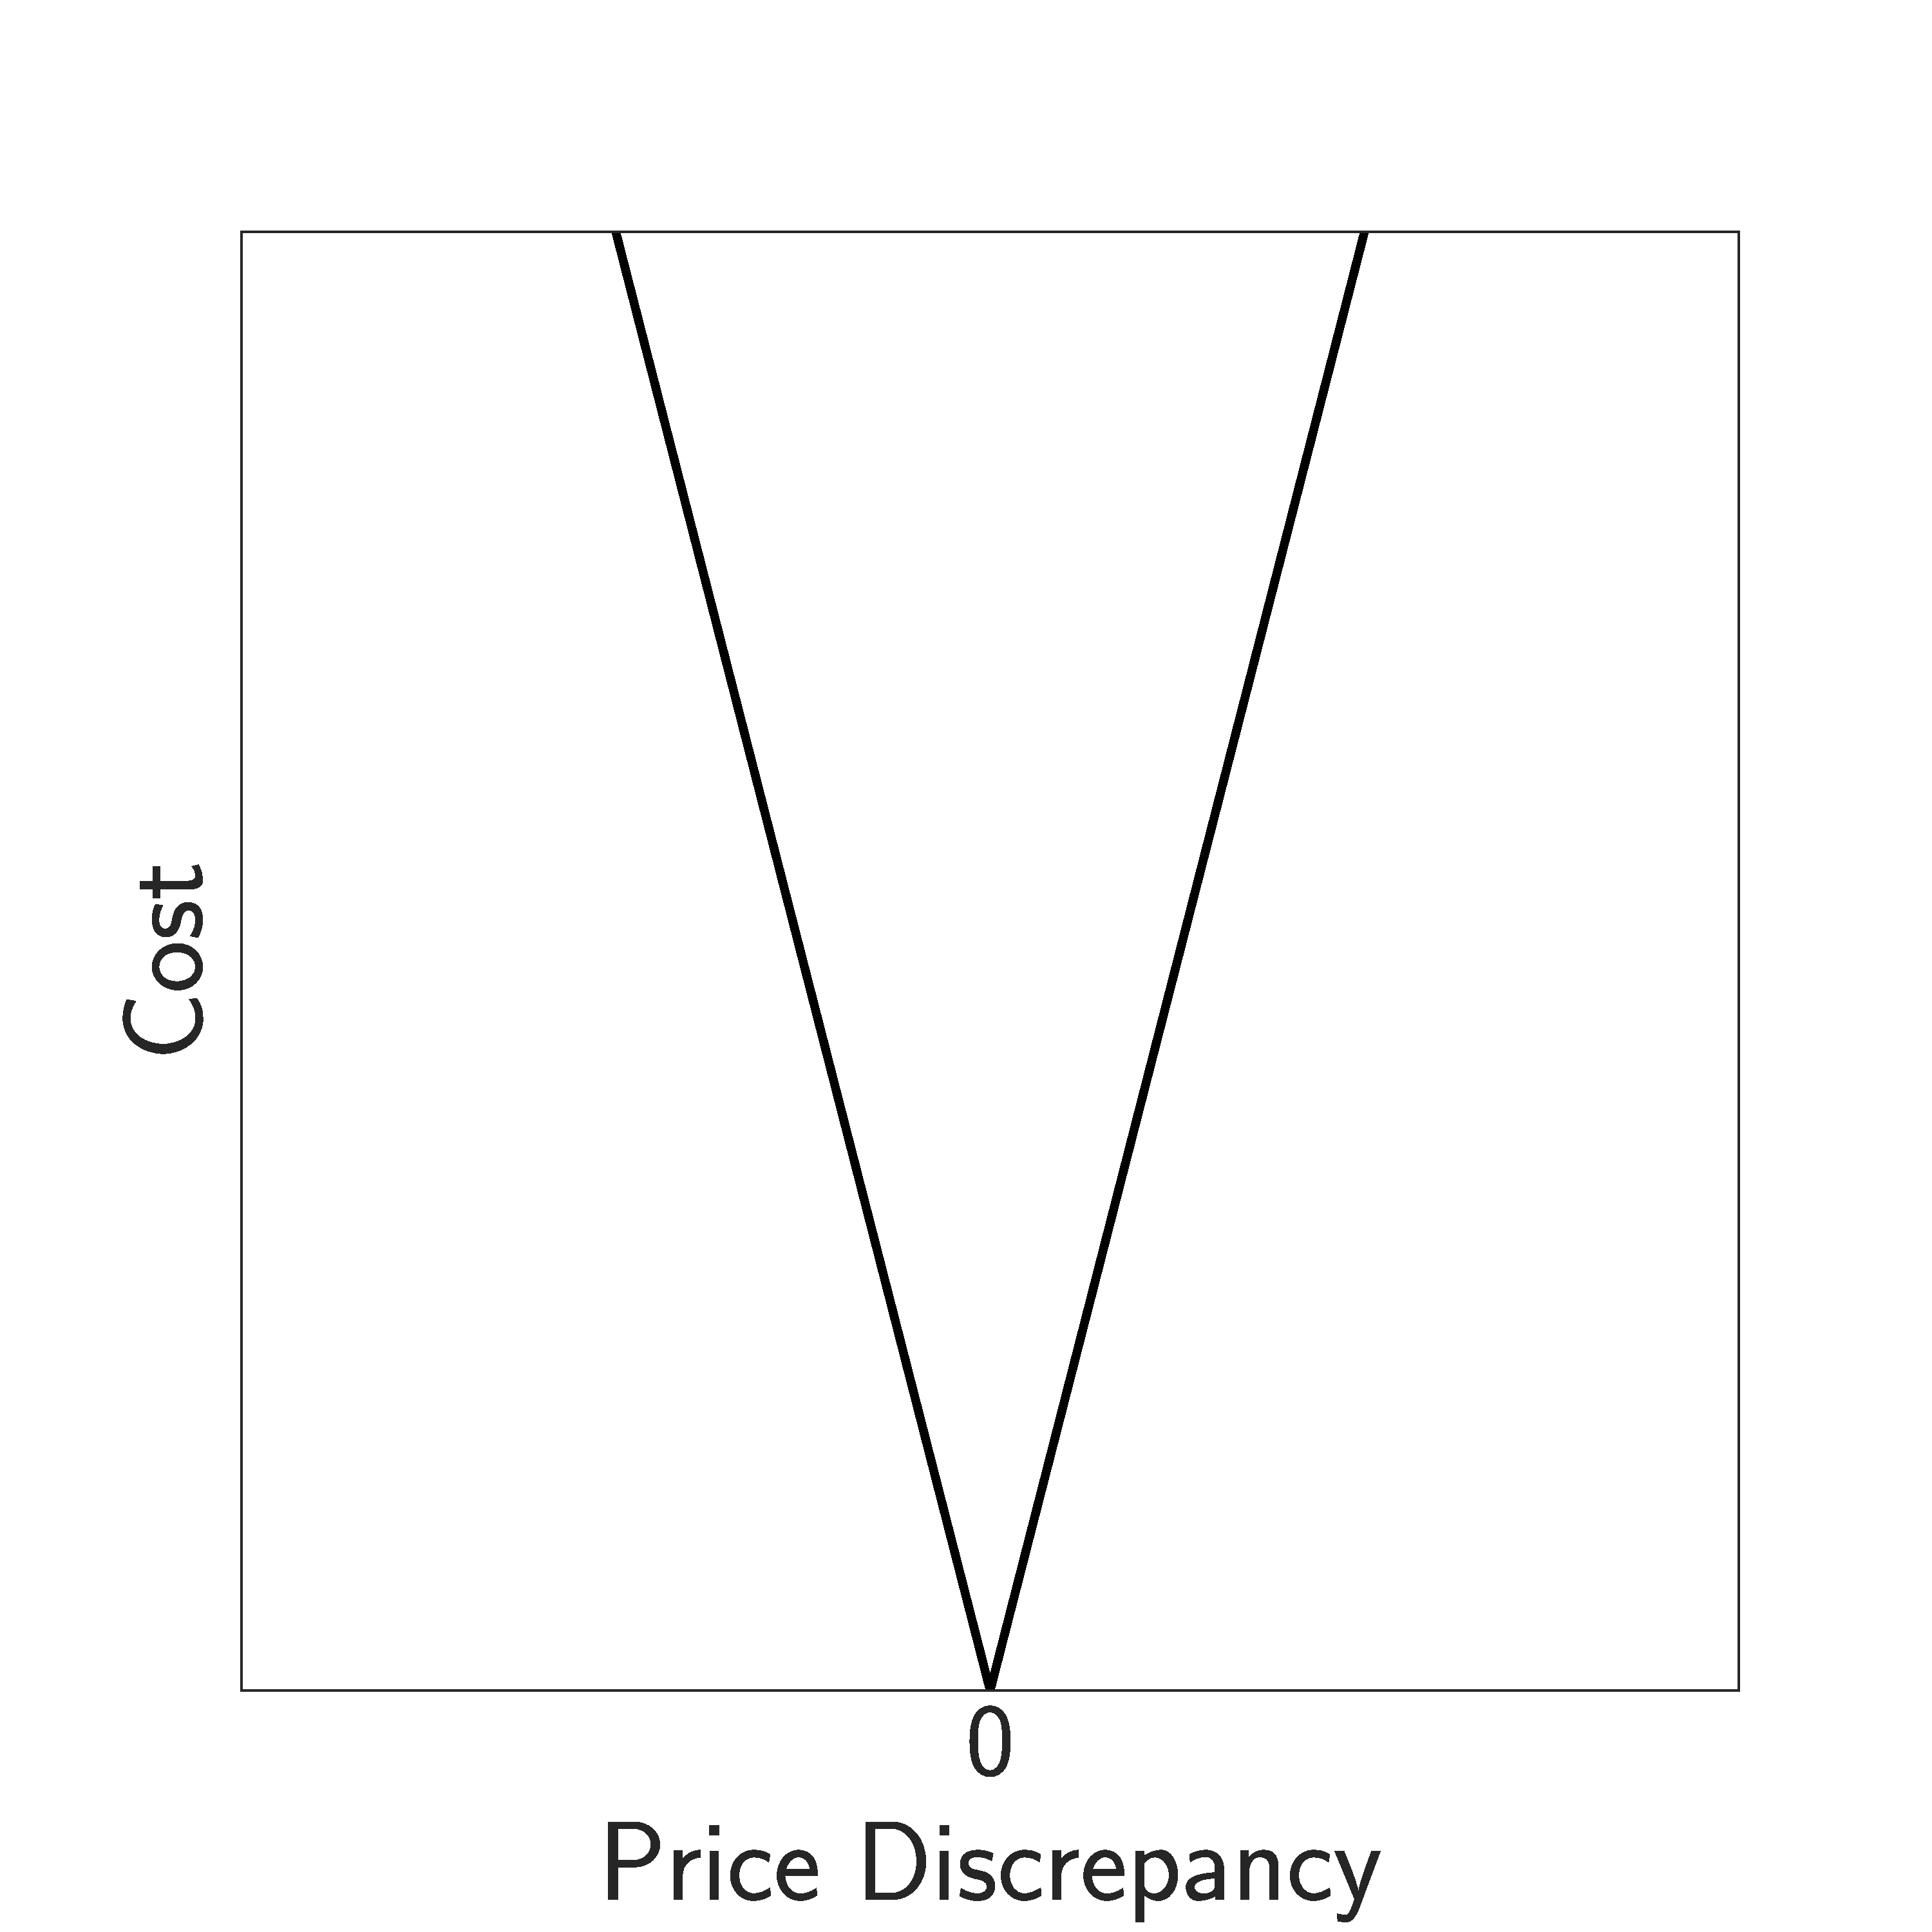
\includegraphics[width=\textwidth]{fig/use-case-leveraged.pdf}
         \caption{leveraged}
         \label{fig:use-case-leveraged}
     \end{subfigure}
     \begin{subfigure}{0.38\textwidth}
         \centering
         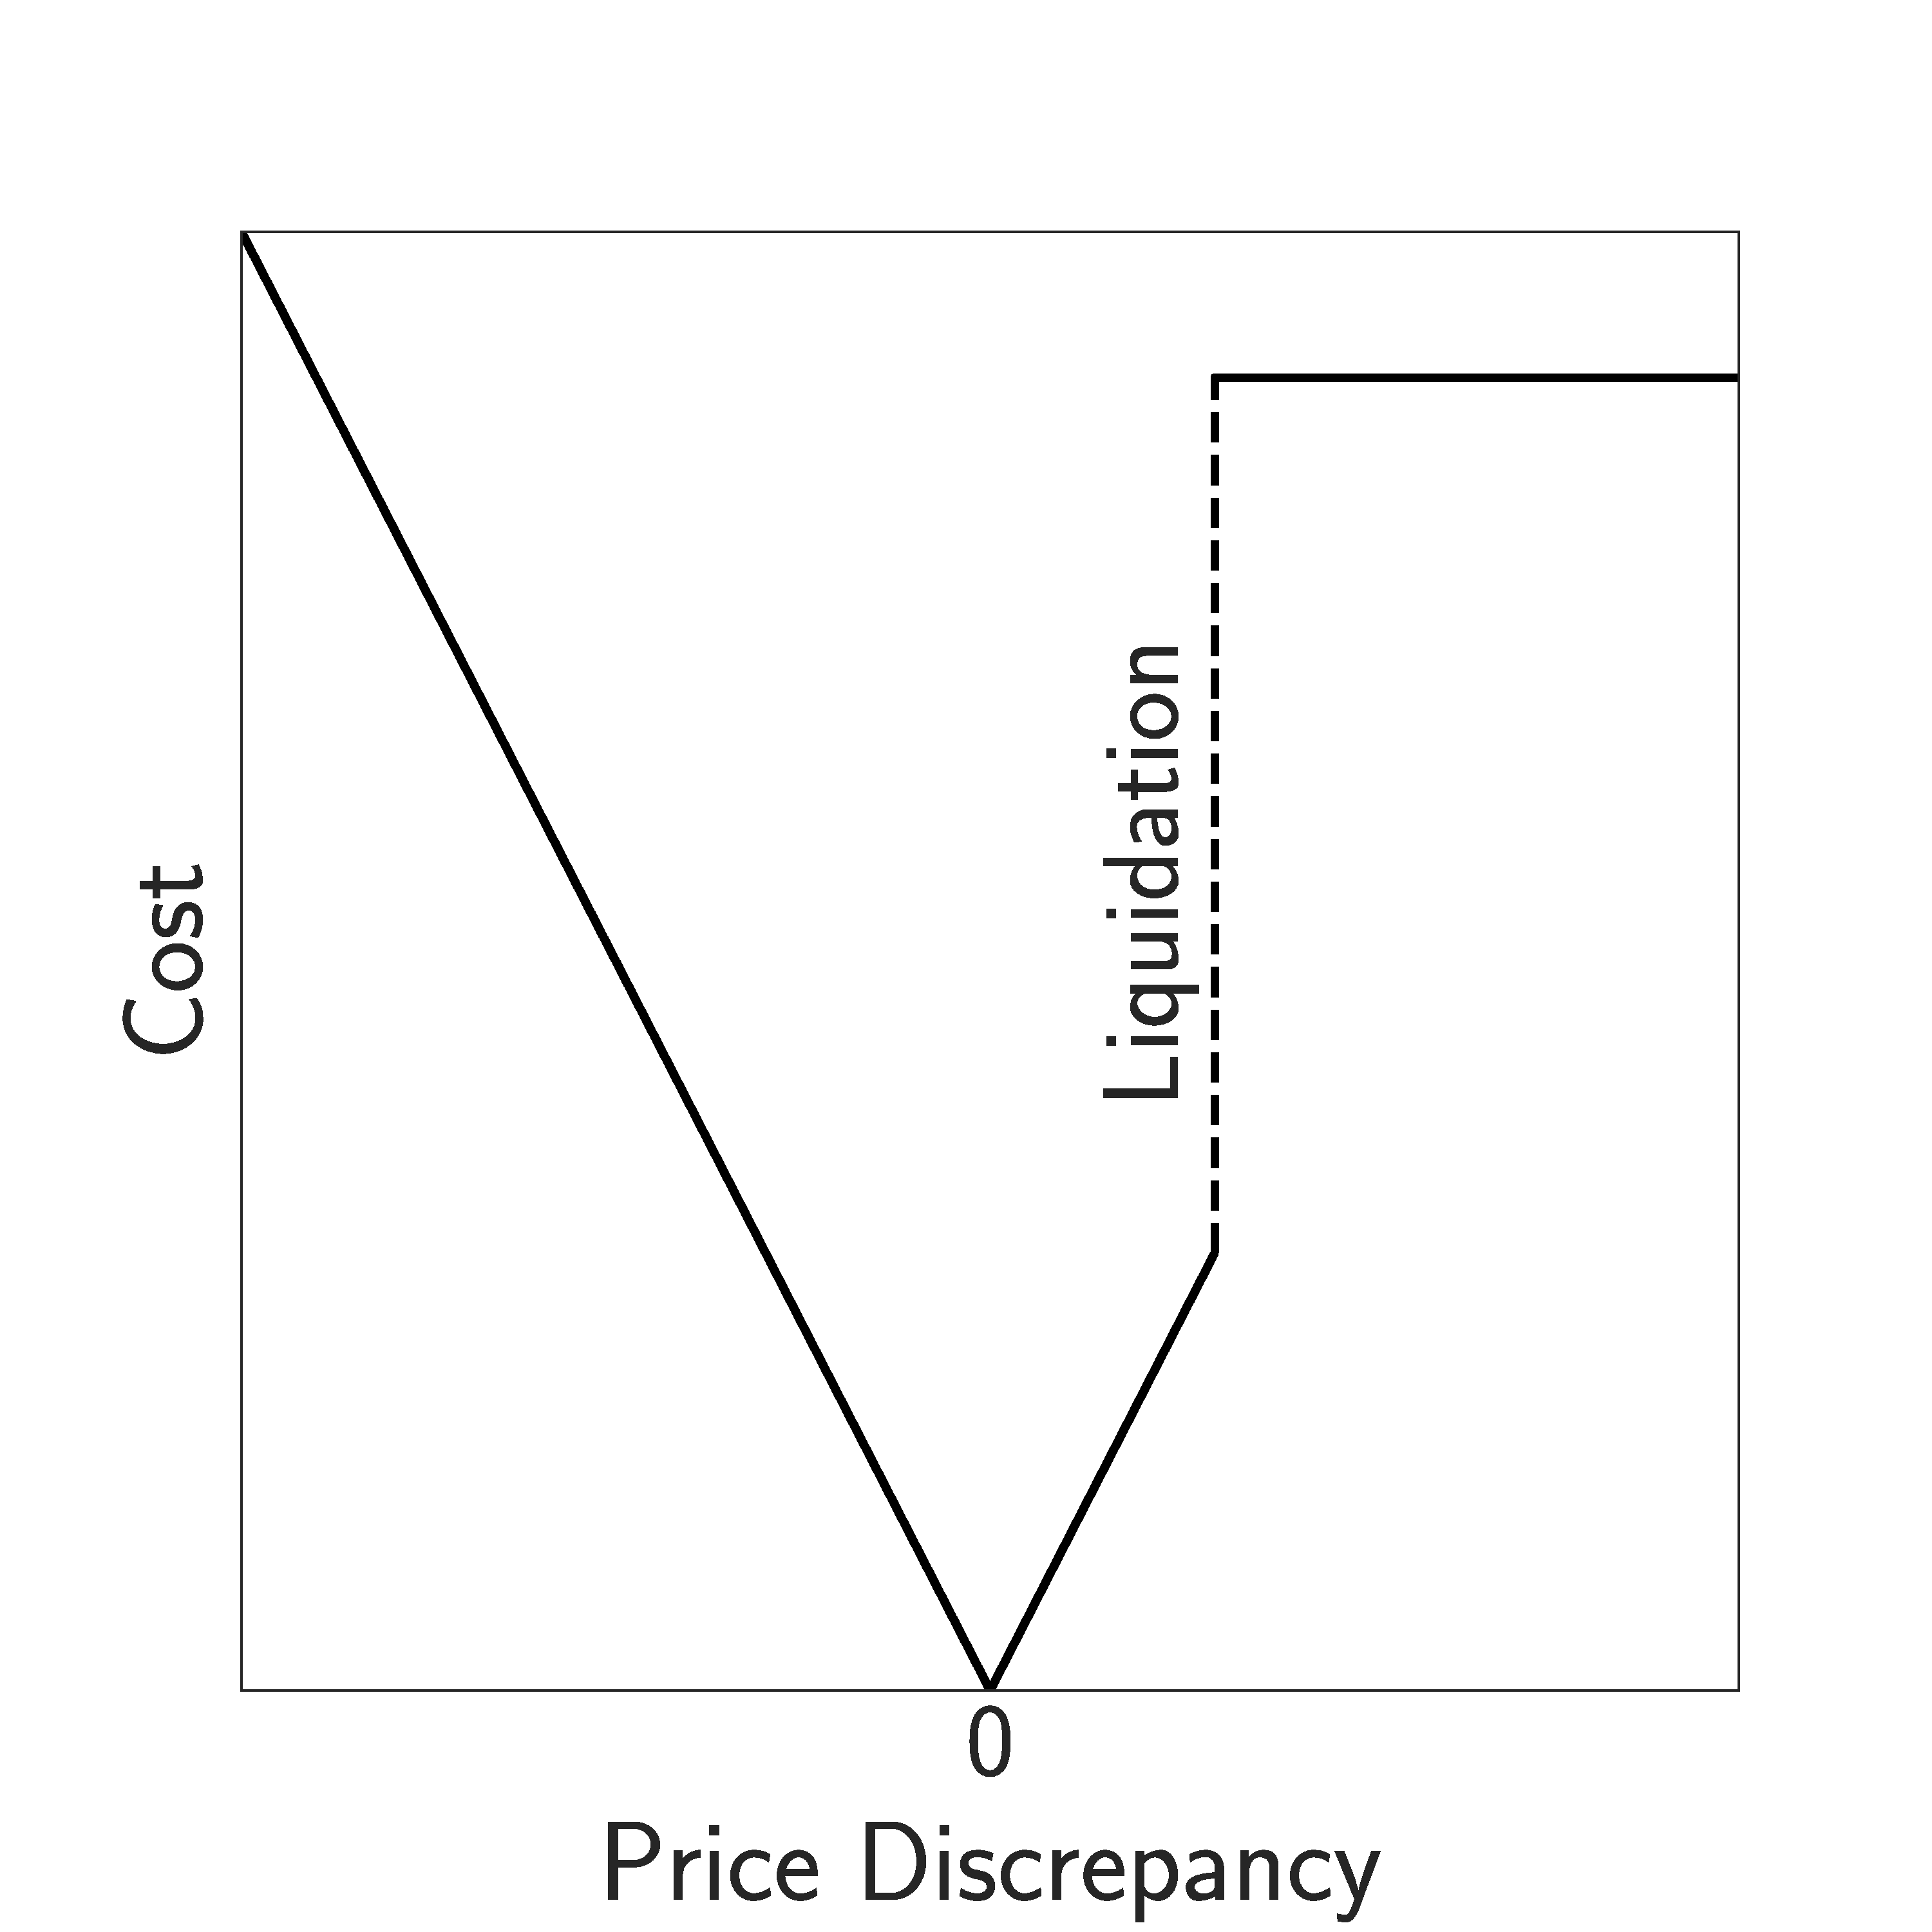
\includegraphics[width=\textwidth]{fig/use-case-discontinuous.pdf}
         \caption{discontinuous, e.g. liquidation}
         \label{fig:use-case-discontinuous}
     \end{subfigure}
    \caption{Los datos de la dAPI pueden utilizarse en diferentes sistemas, y la linealidad y la continuidad en la mecánica de dichos sistemas deciden cuán sensibles son a los errores en los datos de entrada.}
    \label{fig:use-case-types}
\end{figure}

Los factores de riesgo externos determinan el valor esperado de los daños cuando se produce una avería, y la forma en que se utilizan los datos es un aspecto importante de ello. Véase la Figura~\ref{fig:use-case-types}, donde ilustramos el costo de los errores de datos para varias aplicaciones hipotéticas de DeFi.

En la Figura ~\ref{fig:use-case-linear}, la dAPI proporciona datos de precios a una casa de cambio regular, y los errores dan como resultado una ganancia y una pérdida linealmente proporcional para las partes que realizan la transacción (nótese que sólo consideramos las pérdidas). Compárese con la Figura~\ref{fig:use-case-leveraged}, , que representa una casa de cambio con un volumen similar que soporta posiciones apalancadas. Aquí, cualquier error tiene un potencial mucho mayor de causar daños. Por último, véase la Figura ~\ref{fig:use-case-discontinuous}, en la que un usuario ha abierto una posición corta. Una ligera desviación hacia arriba en los datos reportados puede desencadenar una liquidación y causar un efecto desproporcionado. Estos ejemplos indican que es imposible estimar el riesgo de seguro de un usuario específico sin considerar cómo utilizarán exactamente los datos que reciben de la dAPI.

También hay un aspecto más cualitativo del seguro. Concretamente, la API3 y el usuario de la dAPI acordarán una póliza de seguro, en la que se definirán términos como qué es un mal funcionamiento de la dAPI y cómo se calculan los daños. Los jurados de Kleros usarán estas pólizas como referencia para decidir si un reclamo de seguro debe ser pagado. Los términos específicos son importantes en cuanto a la forma de determinar las tasas de seguro. Por ejemplo, el seguro que cubre cualquier fallo de funcionamiento sería más caro que el seguro contra el tiempo de inactividad.

\subsection{Soluciones de escalamiento y seguro}
\label{sec:scaling-solutions-and-insurance}

Casos de uso de alto valor como el DeFi, que se están popularizando, hacen que la red del Ethereum se congestione. Esto aumenta las tarifas de transacción y, como consecuencia, afecta a los costos de operación de la alimentación de datos. Entonces, se vuelve crítico poder hacer uso de soluciones de escalamiento para entregar servicios dAPI a un costo razonable.

Las soluciones de oráculo descentralizadas existentes proponen utilizar soluciones de escalamiento off-chain ~\cite{ellis:2017,band}.
Sin embargo, esas soluciones tienen consecuencias de seguridad poco claras que el usuario no puede evaluar con precisión. En primer lugar, las soluciones de escalado tienden a tener garantías de seguridad más relajadas en general, y no es razonable esperar que el usuario tenga una comprensión sólida de las consecuencias. Además, existen riesgos operacionales adicionales, por ejemplo, problemas de seguridad con la aplicación de una función criptográfica personalizada, la solución de segundo nivel que deniega el servicio, etc. Además, existen riesgos operacionales adicionales, por ejemplo, problemas de seguridad con la aplicación de una función de criptografía personalizada, la solución de segundo nivel que deniega el servicio, etc.  En consecuencia, sería razonable esperar que los usuarios se muestren aprensivos ante la utilización de las fuentes de datos en función de las soluciones de escalamiento.

El seguro dAPI viene como una solución inesperada a este problema debido a su flexibilidad. Si el DAO API3 decide que una solución de escalamiento es de confianza para un caso de uso determinado, la dAPI respectiva puede utilizar esa solución de escalamiento, y su seguro cubriría los posibles daños que causaría la misma. Todo el proceso de reclamación al seguro funcionaría exactamente igual, dado que lo que importa en última instancia es si el servicio se presta correctamente o no al usuario de la dAPI.


\section{Conclusión}
\label{sec:conclusion}

La API3 conectará las aplicaciones descentralizadas con los abundantes datos y servicios que ofrecen las APIs tradicionales de la web, ampliando así la aplicabilidad de la cadena de bloques sin sacrificar la descentralización. Esto se logrará mediante las dAPIs —API totalmente descentralizados y nativos de la cadena de bloques— que serán establecidas, administradas y monetizadas a escala por el DAO API3.

La solución API3 incorpora una variedad de cualidades por diseño.  La más importante de ellas es la \textbf{seguridad}. Las dAPIs no dependen de oráculos de terceros, que son un factor de riesgo constante y significativo en las soluciones alternativas.  Además, el servicio de seguro de dAPI proporciona garantías de seguridad, cuantificables y fiables a sus usuarios, lo que consolida aún más el lugar de la API3 como la solución más segura para recibir servicios de API como aplicación descentralizada.

La segunda cualidad de la solución API3 es su \textbf{robustez} en múltiples niveles. Airnode utiliza tecnología sin servidores, que es muy resistente a los tiempos de inactividad.  Junto con un diseño de nodo sin estado que no se ve fácilmente afectado por errores o condiciones de red adversas, los oráculos API3 están diseñados para ser robustos. Además, las dAPIs se regirán por un DAO que mantiene un equilibrio autorregulado de riesgo y recompensa mediante incentivos bien diseñados, lo que proporciona un marco robusto de mitigación de riesgos.

Las dAPIs eliminan los intermediarios, lo que les otorga su tercera calidad, la  \textbf{rentabilidad}.
No tienen que pagar el impuesto de intermediarios, que es el pago que se hace a los oráculos de terceros para incentivarlos a no intentar un ataque.  Además, las fuentes de datos compuestas por oráculos de primera mano no requieren una redundancia excesiva a esta escala. Al lograr el mismo nivel de descentralización con menos oráculos, las dAPIs proporcionan ahorros muy significativos en los costos de gas.

Por último, la solución API3 logra \textbf{flexibilidad} mediante la completa descentralización de la gestión a partes con verdadera piel en el juego. Por consiguiente, el proyecto nunca se verá limitado por lo que se expone en este documento, y evolucionará constantemente para hacer frente a nuevos desafíos y necesidades.

La primera generación de aplicaciones descentralizadas se limitó a los confines de la cadena de bloques. Hoy en día, tenemos aplicaciones descentralizadas que pueden interactuar con el mundo fuera de la cadena de una manera limitada y pseudo-descentralizada. La API3 impulsará la siguiente ola evolutiva: la tercera generación de aplicaciones descentralizadas que interactúan de forma valiosa con el mundo off-chain, aprovechando las APIs de una forma verdaderamente descentralizada y de mínima confianza.


\small
\bibliographystyle{ieeetr}
\bibliography{refs}

\newpage
\normalsize
\appendix
\section{Glossary}

\textbf{Airnode:} Un nodo oráculo sin servidores diseñado para ser operado por proveedores de API.

\textbf{API:} Una interfaz técnica de una aplicación que otra aplicación puede usar para interactuar con ella por medio de la programación. Una API que está abierta al acceso externo (es decir, una API Web) puede ser utilizada por las empresas para monetizar sus datos y servicios.

\textbf{Proveedor API:} Un negocio que monetiza sus datos y servicios a través de una API.

\textbf{API3:} El proyecto que construirá, administrará y monetizará las dAPIs.

\textbf{DAO API3:} El órgano rector del Proyecto API3.

\textbf{Token API3:} El token que se utiliza para ajustar los incentivos del ecosistema API3. Otorga poder de voto en el DAO API3.

\textbf{ChainAPI:} Una plataforma de integración API-Airnode de terceros. Proporcionará herramientas de integración, servicios públicos y un mercado para la lista pública de puntos finales de oráculo. Puede considerarse como el sucesor espiritual del Mercado API de Honeycomb.

\textbf{DAO:} Organización autónoma descentralizada. Un contrato inteligente multiusuario que se utiliza para democratizar el gobierno de una organización on-chain.

\textbf{dAPI:} Una API descentralizada, es decir, una alimentación de datos compuesta por oráculos de primera mano. Se rige de manera descentralizada por el DAO API3.

\textbf{Mercado API de Honeycomb:} Un servicio de mercado/listado centrado en la API que ha sido construido para los oráculos Chainlink por algunos de los miembros fundadores de la API3.

\textbf{Oráculo:} Un agente que puede entregar datos a y desde una plataforma de contratos inteligentes, por ejemplo, escribe datos de precios de activos a la cadena. Incluye un nodo y un contrato inteligente que implementa el protocolo que utiliza para comunicarse con los solicitantes.

\textbf{Nodo Oráculo:} Una aplicación que realiza las funciones off-chain de un oráculo, por ejemplo, llama a una API para obtener datos de precios de activos y los escribe en la cadena.

\textbf{Web 3.0:} La web descentralizada construida sobre tecnologías de la cadena de bloques. Note que no estamos usando este término para referirnos a la Web Semántica.

\textbf{Web API:} Una API accesible a través de la Web, es decir, una API que no sólo es accesible desde una red privada.

\end{document}

